% !TEX root = saveliev_physics_general_course_2.tex
%!TEX TS-program = pdflatex
%!TEX encoding = UTF-8 Unicode


\chapter{ELECTRIC FIELD IN A VACUUM}\label{chap:1}

\section{Electric Charge}\label{sec:1_1}

All bodies in nature are capable of becoming electrified, \ie, acquiring an electric charge. The presence of such a charge manifests itself in that a charged body interacts with other charged bodies. Two kinds of electric charges exist. They are conventionally called positive and negative. Like charges repel each other, and unlike charges attract each other.

An electric charge is an integral part of certain elementary particles\footnote{Elementary particles are defined as such microparticles whose internal structure at the present level of development of physics cannot be conceived as a combination of other particles.}. The charge of all elementary particles (if it is not absent) is identical in magnitude. It can be called an \textbf{elementary charge}. We shall use the symbol $e$ to denote a positive elementary charge.

The elementary particles include, in particular, the electron (carrying the negative charge $-e$), the proton (carrying the positive charge $+e$), and the neutron (carrying no charge). These particles are the bricks which the atoms and molecules of any substance are built of, therefore all bodies contain electric charges. The particles carrying charges of different signs are usually present in a body in equal numbers and are distributed over it with the same density. The algebraic sum of the charges in any elementary volume of the body equals zero in this case, and each such volume (as well as the body as a whole) will be neutral. If in some way or other we create a surplus of particles of one sign in a body (and, correspondingly, a shortage of particles of the opposite sign), the body will be charged. It is also possible, without changing the total number of positive and negative particles, to cause them to be redistributed in a body so that one part of it has a surplus of charges of one sign and the other part a surplus of charges of the opposite sign. This can be done by bringing a charged body close to an uncharged metal one.

Since a charge $q$ is formed by a plurality of elementary charges, it is an integral multiple of $e$:
\begin{equation}\label{eq:1_1}
	q = \pm N e.
\end{equation}

\noindent
An elementary charge is so small, however, that macroscopic charges may be considered to have continuously changing magnitudes.

If a physical quantity can take on only definite discrete values, it is said to be quantized. The fact expressed by \eqn{1_1} signifies that an electric charge is quantized.

The magnitude of a charge measured in different inertial reference frames will be found to be the same. Hence, an electric charge is relativistically invariant. It thus follows that the magnitude of a charge does not depend on whether the charge is moving or at rest.

Electric charges can vanish and appear again. Two elementary charges of opposite signs always appear or vanish simultaneously, however. For example, an electron and a positron (a positive electron) meeting each other annihilate, \ie, transform into neutral gamma-photons. This is attended by vanishing of the charges $-e$ and $+e$. In the course of the process called the birth of a pair, a gamma-photon getting into the field of an atomic nucleus transforms into a pair of particles---an electron and a positron. This process causes the charges $-e$ and $+e$ to appear.

Thus, the total charge of an electrically isolated system\footnote{A system is referred to as electrically isolated if no charged particles can penetrate through the surface confining it.} cannot change. This statement forms the \textbf{law of electric charge conservation}.

We must note that the law of electric charge conservation is associated very closely with the relativistic invariance of a charge. Indeed, if the magnitude of a charge depended on its velocity, then by bringing charges of one sign into motion we would change the total charge of the relevant isolated system.

\section{Coulomb's Law}\label{sec:1_2}

The law obeyed by the force of interaction of point charges was established experimentally in 1785 by the French physicist Charles A. de Coulomb (1736-1806). A \textbf{point charge} is defined as a charged body whose dimensions may be disregarded in comparison with the distances from this body to other bodies carrying an electric charge.

Using a torsion balance (\fig{1_1}) similar to that employed by H. Cavendish to determine the gravitational constant (see Vol. I, Sec. 6.1), Coulomb measured the force of interaction of two charged spheres depending on the magnitude of the charges on them and on the distance between them. He proceeded from the fact that when a charged metal sphere was touched by an identical uncharged sphere, the charge would be distributed equally between the two spheres.

\begin{figure}[t]
	\begin{center}
		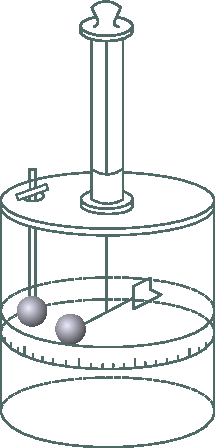
\includegraphics[scale=0.9]{figures/ch_01/fig_1_1.pdf}
		\caption[]{}
		\label{fig:1_1}
	\end{center}
	\vspace{-0.8cm}
\end{figure}

As a result of his experiments, Coulomb arrived at the conclusion that \textit{the force of interaction between two stationary point charges is proportional to the magnitude of each of them and inversely proportional
to the square of the distance between them}. The direction of the force coincides with the straight line connecting the charges.

It must be noted that the direction of the force of interaction along the straight line connecting the point charges follows from considerations of symmetry. An empty space is assumed to be homogeneous and isotropic. Consequently, the only direction distinguished in the space by stationary point charges introduced into it is that from one charge to the other. Assume that the force $\vec{F}$ acting on the charge $q_i$ (\fig{1_2}) makes the angle $\alpha$ with the direction from $q_1$ to $q_2$, and that $\alpha$ differs from $0$ or $\pi$. But owing to axial symmetry, there are no grounds to set the force $\vec{F}$ aside from the multitude of forces of other directions making the same angle $\alpha$ with the axis $q_1$-$q_2$ (the directions of these forces form a cone with a cone angle of $2\alpha$). The difficulty appearing as a result of this vanishes when $\alpha$ equals $0$ or $\pi$.

\begin{figure}[t]
	\begin{minipage}[t]{0.5\linewidth}
		\begin{center}
			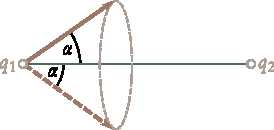
\includegraphics[scale=1]{figures/ch_01/fig_1_2.pdf}
			\caption[]{}
			\label{fig:1_2}
		\end{center}
	\end{minipage}
	\hspace{-0.05cm}
	\begin{minipage}[t]{0.5\linewidth}
		\begin{center}
			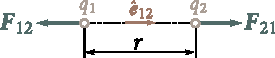
\includegraphics[scale=1]{figures/ch_01/fig_1_3.pdf}
			\caption[]{}
			\label{fig:1_3}
		\end{center}
	\end{minipage}
\vspace{-0.4cm}
\end{figure}

Coulomb's law can be expressed by the formula
\begin{equation}\label{eq:1_2}
	\vec{F}_{12} = -k \frac{q_1 q_2}{r^2}\,\vecuni{12}.
\end{equation}

\noindent
Here, $k$ is a proportionality constant assumed to be positive, $q_1$ and $q_2$ are magnitudes of the interacting charges, $r$ is the distance between the charges, $\vecuni{12}$ is the unit vector directed from the charge $q_1$ to $q_2$ and $\vec{F}_{12}$ is the force acting on the charge $q_1$ (\fig{1_3}; the figure corresponds to the case of like charges).

The force $\vec{F}_{21}$ differs from $\vec{F}_{12}$ in its sign:
\begin{equation}\label{eq:1_3}
	\vec{F}_{21} = k \frac{q_1 q_2}{r^2}\,\vecuni{12}.
\end{equation}

The magnitude of the interaction force, which is the same for both charges, can be written in the form
\begin{equation}\label{eq:1_4}
	F = k \frac{\absolute{q_1 q_2}}{r^2}.
\end{equation}

Experiments show that the force of interaction between two given charges does not change if other charges are placed near them. Assume that we have the charge $\ab{q}{a}$ and, in addition, $N$ other charges $q_1, q_2,\ldots, q_N$. It can be seen from the above that the resultant force $\vec{F}$ with which all the $N$ charges $q_i$ act on $\ab{q}{a}$ is
\begin{equation}\label{eq:1_5}
	\vec{F} = \sum_{i=1}^N \ab{\vec{F}}{a, $i$}
\end{equation}

\noindent
where $\ab{\vec{F}}{a, $i$}$ is the force with which the charge $q_i$ acts on $\ab{q}{a}$ in the absence of the other $N-1$ charges.

The fact expressed by \eqn{1_5} permits us to calculate the force of interaction between charges concentrated on bodies of finite dimensions, knowing the law of interaction between point charges. For this purpose, we must divide each charge into so small charges $\deriv{q}$ that they can be considered as point ones, use \eqn{1_2} to calculate the force of interaction between the charges $\deriv{q}$ taken in pairs, and then perform vector summation of these forces. Mathematically, this procedure coincides completely with the calculation of the force of gravitational attraction between bodies of finite dimensions (see Vol. I, Sec. 6.1).

All experimental facts available lead to the conclusion that Coulomb's law holds for distances from \SI{e-15}{\metre} to at least several kilometres. There are grounds to presume that for distances smaller than \SI{e-16}{\metre} the law stops being correct. For very great distances, there are no experimental confirmations of Coulomb's law. But there are also no reasons to expect that this law stops being obeyed with very great distances between charges.

\section{Systems of Units}\label{sec:1_3}

We can make the proportionality constant in \eqn{1_2} equal unity by properly choosing the unit of charge (the units for $F$ and $r$ were established in mechanics). The relevant unit of charge (when $F$ and $r$ are measured in cgs units) is called the \textbf{absolute electrostatic unit} of charge (cgse$_q$). It is the magnitude of a charge that interacts with a force of \SI{1}{\dyne} in a vacuum with an equal charge at a distance of \SI{1}{\centi\metre} from it.

Careful measurements (they are described in~\sect{10_3}) showed that an elementary charge is
\begin{equation}\label{eq:1_6}
	e = \num{4.80e-10}\text{ cgse$_q$}.
\end{equation}

Adopting the units of length, mass, time, and charge as the basic ones, we can construct a system of units of electrical and magnetic quantities. The system based on the centimetre, gramme, second, and the cgse$_q$ unit is called the \textbf{absolute electrostatic system of units} (the cgse system). It is founded on Coulomb's law, \ie, the law of interaction between charges at rest. On a later page, we shall become acquainted with the \textbf{absolute electromagnetic system of units} (the cgsm system) based on the law of interaction between conductors carrying an electric current. The Gaussian system in which the units of electrical quantities coincide with those of the cgse system, and of magnetic quantities with those of the cgsm system, is also an absolute system.

Equation~\eqref{eq:1_4} in the cgse system becomes
\begin{equation}\label{eq:1_7}
	F = \frac{\absolute{q_1 q_2}}{r^2}.
\end{equation}

\noindent
This equation is correct if the charges are in a vacuum. It has to be determined more accurately for charges in a medium (see \sect{2_8}).

USSR State Standard GOST 9867-61, which came into force on January 1, 1963, prescribes the preferable use of the International System of Units (SI). The basic units of this system are the metre, kilogramme, second, ampere, kelvin, candela, and mole. The SI unit of force is the newton (\si{\newton}) equal to \num{e5} dynes.

In establishing the units of electrical and magnetic quantities, the SI system, like the cgsm one, proceeds from the law of interaction of current-carrying conductors instead of charges. Consequently, the proportionality constant in the equation of Coulomb's law is a quantity with a dimension and differing from unity.

The SI unit of charge is the coulomb (\si{\coulomb}). It has been found experimentally that
% \vspace{-12pt}
\begin{equation}\label{eq:1_8}
	\SI{1}{\coulomb} = \num{2.998e9} \approx \num{3e9}{\text{ cgse$_q$}}.
\end{equation}

To form an idea of the magnitude of a charge of \SI{1}{\coulomb}, let us calculate the force with which two point charges of \SI{1}{\coulomb} each would interact with each other if they were \SI{1}{\metre} apart. By \eqn{1_7}
\begin{equation}\label{eq:1_9}
	F = \frac{\num{3e9}\times\num{3e9}}{100^2}\,\text{ cgse$_F$} = \SI{9e14}{\dyne} = \SI{9e9}{\newton} \approx \SI{e9}{\kgf}.
\end{equation}

An elementary charge expressed in coulombs is
\begin{equation}\label{eq:1_10}
	e = \SI{1.60e-19}{\coulomb}.
\end{equation}

\section{Rationalized Form of Writing Formulas}\label{sec:1_4}

Many formulas of electrodynamics when written in the cgs systems (in particular, in the Gaussian one) include as factors $4\pi$ and the so-called electromagnetic constant $c$ equal to the speed of light in a vacuum. To eliminate these factors in the formulas that are most important in practice, the proportionality constant in Coulomb's law is taken equal to $1/4\pi\varepsilon_0$. The equation of the law for charges in a vacuum will thus become
\begin{equation}\label{eq:1_11}
	F = \frac{1}{4\pi\varepsilon_0}\frac{\absolute{q_1 q_2}}{r^2}.
\end{equation}

\noindent
The other formulas change accordingly. This modified way of writing formulas is called \textbf{rationalized}. Systems of units constructed with the use of rationalized formulas are also called \textbf{rationalized}. They include the SI system.

The quantity $\varepsilon_0$ is called the \textbf{electric constant}. It has the dimension of capacitance divided by length. It is accordingly expressed in units called the farad per metre. To find the numerical value of $\varepsilon_0$, we shall introduce the values of the quantities corresponding to the case of two charges of \SI{1}{\coulomb} each and \SI{1}{\metre} apart into \eqn{1_11}. By \eqn{1_9}, the force of interaction in this case is \SI{9e9}{\newton}. Using this value of the force, and also $q_1=q_2=\SI{1}{\coulomb}$ and $r=\SI{1}{\metre}$ in \eqn{1_11}, we get
\begin{equation*}
	\num{9e9} = \frac{1}{4\pi\varepsilon_0}\frac{\absolute{1\times 1}}{1^2}
\end{equation*}

\noindent
whence
\begin{equation}\label{eq:1_12}
	\varepsilon_0 = \frac{1}{4\pi\times\num{9e9}} = \SI{0.885e-11}{\faraday\per\metre}.
\end{equation}

The Gaussian system of units was widely used and is continuing to be used in physical publications. We therefore consider it essential to acquaint our reader with both the SI and the Gaussian system. We shall set out the material in the SI units showing at the same time how the formulas look in the Gaussian system. The fundamental formulas of electrodynamics written in the SI and the Gaussian system are compared in \app{A_3}.

\section{Electric Field. Field Strength}\label{sec:1_5}

Charges at rest interact through an electric field\footnote{We shall see in \sect{6_2} that when considering moving charges, their interaction in addition to an electric field is due to a magnetic field.}. A charge alters the properties of the space surrounding it---it sets up an electric field in it. This field manifests itself in that an electric charge placed at a point of it experiences the action of a force. Hence, to see whether there is an electric field at a given place, we must place a charged body (in the following we shall say simply a charge for brevity) at it and determine whether or not it experiences the action of an electric force. We can evidently assess the ``strength'' of the field according to the magnitude of the force exerted on the given charge.

Thus, to detect and study an electric field, we must use a ``test'' charge. For the force acting on our test charge to characterize the field ``at the given point'', the test charge must be a point one. Otherwise, the force acting on the charge will characterize the properties of the field averaged over the volume occupied by the body that carries the test charge.

\begin{figure}[t]
	\begin{center}
		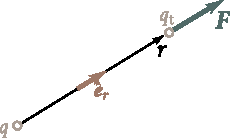
\includegraphics[scale=1]{figures/ch_01/fig_1_4.pdf}
		\caption[]{}
		\label{fig:1_4}
	\end{center}
	\vspace{-0.8cm}
\end{figure}

Let us study the field set up by the stationary point charge $q$ with the aid of the point test charge $\ab{q}{t}$. We place the test charge at a point whose position relative to the charge $q$ is determined by the position vector $\vec{r}$ (\fig{1_4}). We see that the test charge experiences the force
\begin{equation}\label{eq:1_13}
	\vec{F} = \ab{q}{t} \parenthesis{
	\frac{1}{4\pi\varepsilon_0} \frac{q}{r^2}\,\vecuni{r}
	}
\end{equation}

\noindent
[see Eqs. \eqref{eq:1_3} and \eqref{eq:1_11}]. Here $\vecuni{r}$ is the unit vector of the position vector $\vec{r}$.

A glance at \eqn{1_13} shows that the force acting on our test charge depends not only on the quantities determining the field (on $q$ and $\vec{r}$), but also on the magnitude of the test charge $\ab{q}{t}$. If we take different test charges $\ab{q}{t}'$, $\ab{q}{t}''$, etc., then the forces $\vec{F}'$, $\vec{F}''$, etc. which they experience at the given point of the field will be different.
We can see from \eqn{1_13}, however, that the ratio $F/\ab{q}{t}$ for all the test charges will be the same and depend only on the values of $q$ and $\vec{r}$ determining the field at the given point. It is therefore natural to adopt this ratio as the quantity characterizing an electric field:
\begin{equation}\label{eq:1_14}
	\vec{E} = \frac{\vec{F}}{\ab{q}{t}}.
\end{equation}

\noindent
This vector quantity is called the \textbf{electric field strength} (or \textbf{intensity}) at a given point (\ie, at the point where the test charge $\ab{q}{t}$ experiences the action of the force $\vec{F}$).

According to \eqn{1_14}, the electric field strength numerically equals the force acting on a unit point charge at the given point of the field. The direction of the vector $\vec{E}$ coincides with that of the force acting on a positive charge.

It must be noted that \eqn{1_14} also holds when the test charge is negative ($\ab{q}{t}<0$). In this case, the vectors $\vec{E}$ and $\vec{F}$ have opposite directions.

We have arrived at the concept of electric field strength when studying the field of a stationary point charge. Definition \eqref{eq:1_14}, however, also covers the case of a field set up by any collection of stationary charges, but here the following clarification is needed. The arrangement of the charges setting up the field being studied may change under the action of the test charge. This will happen, for example, when the charges producing the field are on a conductor and can freely move within its limits. Therefore, to avoid appreciable alterations in the field being studied, a sufficiently small test charge must be taken.

It follows from Eqs. \eqref{eq:1_13} and \eqref{eq:1_14} that the field strength of a point charge varies directly with the magnitude of the charge $q$ and inversely with the square of the distance $r$ from the charge to the given point of the field:
\begin{equation}\label{eq:1_15}
	\vec{E} = \frac{1}{4\pi\varepsilon_0} \frac{q}{r^2}\, \vecuni{r}.
\end{equation}

\noindent
The vector $\vec{E}$ is directed along the radial straight line passing through the charge and the given point of the field, from the charge if the latter is positive and toward the charge if it is negative.

In the Gaussian system, the equation for the field strength of a point charge in a vacuum has the form
\begin{equation}\label{eq:1_16}
	\vec{E} = \frac{q}{r^2}\, \vecuni{r}.
\end{equation}

The unit of electric field strength is the strength at a point where unit force (\SI{1}{\newton} in the SI and \SI{1}{\dyne} in the Gaussian system) acts on unit charge (\SI{1}{\coulomb} in the SI and \num{1}\cgse{q} in the Gaussian system). This unit has no special name in the Gaussian system. The SI unit of electric field strength is called the volt per metre (\si{\volt\per\metre}) [see \eqn{1_44}].

According to \eqn{1_15}, a charge of \SI{1}{\coulomb} produces the following field strength in a vacuum at a distance of \SI{1}{\metre} from this charge:
\begin{equation*}
	E = \frac{1}{4\pi\parenthesis{1/4\pi \times \num{9e9}}} \frac{1}{1^2} = \SI{9e9}{\volt\per\metre}.
\end{equation*}

This strength in the Gaussian system is
\begin{equation*}
	E = \frac{q}{r^2} = \frac{\num{3e9}}{100^2} = \num{3e5}\cgse{E}.
\end{equation*}

\noindent
Comparing these two results, we find that
\begin{equation}\label{eq:1_17}
	1\cgse{E} = \SI{3e4}{\volt\per\metre}.
\end{equation}

According to \eqn{1_14}, the force exerted on a test charge is
\begin{equation*}
	\vec{F} = \ab{q}{t} \vec{E}.
\end{equation*}

\noindent
It is obvious that any point charge $q$\footnote{In \eqn{1_15}, $q$ stands for the charge setting up the field. In \eqn{1_18}, $q$ stands for the charge experiencing the force $\vec{F}$ at a point of strength $\vec{E}$.} at a point of a field with the strength $\vec{E}$ will experience the force
\begin{equation}\label{eq:1_18}
	\vec{F} = q \vec{E}.
\end{equation}

\noindent
If the charge $q$ is positive, the direction of the force coincides with that of the vector $\vec{E}$. If $q$ is negative, the vectors $\vec{F}$ and $\vec{E}$ are directed oppositely.

We mentioned in \sect{1_2} that the force with which a system of charges acts on a charge not belonging to the system equals the vector sum of the forces which each of the charges of the system exerts separately on the given charge [see \eqn{1_15}]. Hence it follows that \textit{the field strength of a system of charges equals the vector sum of the field strengths that would be produced by each of the charges of the system separately}:
\vspace{-12pt}
\begin{equation}\label{eq:1_19}
	\vec{E} = \sum_i \vec{E}_i.
\end{equation}

\noindent
This statement is called the \textbf{principle of electric field superposition}.

The superposition principle allows us to calculate the field strength of any system of charges. By dividing extended charges into sufficiently
small fractions $\deriv{q}$, we can reduce any system of charges to a collection of point charges. We calculate the contribution of each of such charges to the resultant field by \eqn{1_15}.

An electric field can be described by indicating the magnitude and direction of the vector $\vec{E}$ for each of its points. The combination of these vectors forms the field of the electric field strength vector (compare with the field of the velocity vector, Vol. I, Sec. 9.1). The velocity vector field can be represented very illustratively with the aid of flow lines. Similarly, an electric field can be described with the aid of strength lines, which we shall call for short $\vec{E}$ lines or field lines. These lines are drawn so that a tangent to them at every point coincides with the direction of the vector $\vec{E}$. The density of the lines is selected so that their number passing through a unit area at right angles to the lines equals the numerical value of the vector $\vec{E}$. Hence, the pattern of field lines permits us to assess the direction and magnitude of the vector $\vec{E}$ at various points of space (\fig{1_5}).

\begin{figure}[t]
	\begin{minipage}[t]{0.5\linewidth}
		\begin{center}
			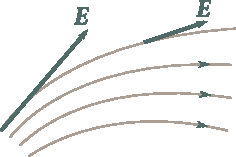
\includegraphics[scale=1]{figures/ch_01/fig_1_5.pdf}
			\caption[]{}
			\label{fig:1_5}
		\end{center}
	\end{minipage}
	\hspace{-0.05cm}
	\begin{minipage}[t]{0.5\linewidth}
		\begin{center}
			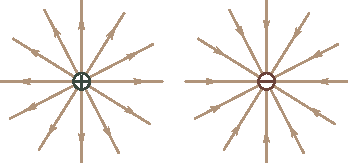
\includegraphics[scale=1]{figures/ch_01/fig_1_6.pdf}
			\caption[]{}
			\label{fig:1_6}
		\end{center}
	\end{minipage}
\vspace{-0.4cm}
\end{figure}

The $\vec{E}$ lines of a point charge field are a collection of radial straight lines directed away from the charge if it is positive and toward it if it is negative (\fig{1_6}). One end of each line is at the charge, and the other extends to infinity. Indeed, the total number of lines intersecting a spherical surface of arbitrary radius $r$ will equal the product of the density of the lines and the surface area of the sphere $4\pi r^2$. We have assumed that the density of the lines numerically equals $E=(1/4\pi\varepsilon_0)(q/r^2)$. Hence, the number of lines is $(1/4\pi\varepsilon_0)(q/r^2) 4\pi r^2=q/\varepsilon_0$. This result signifies that the number of lines at any distance from a charge will be the same. It thus follows hat the lines do not begin and do not terminate anywhere except tor the charge. Beginning at the charge, they extend to infinity (the charge is positive), or arriving from infinity, they terminate at the charge (the latter is negative). This property of the $\vec{E}$ lines is common for all electrostatic fields, \ie, fields set up by any system of stationary charges: the field lines can begin or terminate only at charges or extend to infinity.

\section{Potential}\label{sec:1_6}

Let us consider the field produced by a stationary point charge $q$. At any point of this field, the point charge $q'$ experiences the force
\begin{equation}\label{eq:1_20}
	\vec{F} = \frac{1}{4\pi\varepsilon_0}\frac{qq'}{r^2}\, \vecuni{r} = F(r)\vecuni{r}.
\end{equation}

\noindent
Here $F(r)$ is the magnitude of the force $\vec{F}$, and $\vecuni{r}$ is the unit vector of the position vector $\vec{r}$ determining the position of the charge $q'$ relative to the charge $q$.

\begin{figure}[t]
	\begin{center}
		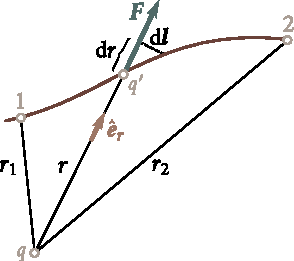
\includegraphics[scale=1]{figures/ch_01/fig_1_7.pdf}
		\caption[]{}
		\label{fig:1_7}
	\end{center}
	\vspace{-0.8cm}
\end{figure}

The force \eqref{eq:1_20} is a central one (see Vol. I, Sec. 3.4). A central field of forces is conservative. Consequently, the work done by the forces of the field on the charge $q'$ when it is moved from one point to another does not depend on the path. This work is
\begin{equation}\label{eq:1_21}
	A_{12} = \int_1^2 F(r) \vecuni{r}\, \deriv{\vec{l}}
\end{equation}

\noindent
where $\deriv{\vec{l}}$ is the elementary displacement of the charge $q'$. Inspection of \fig{1_7} shows that the scalar product $\vecuni{r}\,\deriv{\vec{l}}$ equals the increment of the magnitude of the position vector $\vec{r}$, \ie, $\deriv{r}$. Equation \eqref{eq:1_21} can therefore be written in the form
\begin{equation*}
	A_{12} = \int_1^2 F(r)\, \deriv{r}
\end{equation*}

\noindent
[compare with Eq. (3.24) of Vol. I]. Introduction of the expression for $F(r)$ yields
\begin{equation}\label{eq:1_22}
	A_{12} = \frac{qq'}{4\pi\varepsilon_0} \int_{r_1}^{r_2} \frac{\deriv{r}}{r^2} = \frac{1}{4\pi\varepsilon_0} \parenthesis{
	\frac{qq'}{r_1} - \frac{qq'}{r_2}
	}.
\end{equation}

The work of the forces of a conservative field can be represented as a decrement of the potential energy:
\begin{equation}\label{eq:1_23}
	A_{12} = \ab{W}{p,$1$} - \ab{W}{p,$2$}.
\end{equation}

\noindent
A comparison of Eqs. \eqref{eq:1_22} and \eqref{eq:1_23} leads to the following expression for the potential energy of the charge $q'$ in the field of the charge $q$:
\begin{equation*}
	\ab{W}{p} = \frac{1}{4\pi\varepsilon_0} \frac{qq'}{r_2} + \text{constant}.
\end{equation*}

\noindent
The value of the constant in the expression for the potential energy is usually chosen so that when the charge moves away to infinity (\ie, when $r=\infty$), the potential energy vanishes. When this condition is observed, we get
\begin{equation}\label{eq:1_24}
	\ab{W}{p} = \frac{1}{4\pi\varepsilon_0} \frac{qq'}{r_2}.
\end{equation}

Let us use the charge $q'$ as a test charge for studying the field. By \eqn{1_24}, the potential energy which the test charge has depends not only on its magnitude $q'$, but also on the quantities $q$ and $r$ determining the field. Thus, we can use this energy to describe the field just like we used the force acting on the test charge for this purpose.

Different test charges $\ab{q}{t}'$, $\ab{q}{t}''$, etc. will have different energies $\ab{W}{p}'$, $\ab{W}{p}''$, etc. at the same point of a field. But the ratio $\ab{W}{p}/\ab{q}{t}$ will be the same for all the charges [see \eqn{1_24}]. The quantity
\begin{equation}\label{eq:1_25}
	\varphi = \frac{\ab{W}{p}}{\ab{q}{t}}
\end{equation}

\noindent
is called the \textbf{field potential} at a given point and is used together with the field strength $\vec{E}$ to describe electric fields.

It can be seen from \eqn{1_25} that the potential numerically equals the potential energy which a unit positive charge would have at the given point of the field. Substituting for the potential energy in \eqn{1_25} its value from \eqref{eq:1_24}, we get the following expression for the potential of a point charge:
\begin{equation}\label{eq:1_26}
	\varphi = \frac{1}{4\pi\varepsilon_0} \frac{q}{r}.
\end{equation}

In the Gaussian system, the potential of the field of a point charge in a vacuum is determined by the formula
\begin{equation}\label{eq:1_27}
	\varphi = \frac{q}{r}.
\end{equation}

Let us consider the field produced by a system of $N$ point charges $q_1, q_2,\ldots, q_N$. Let $r_1, r_2,\ldots, r_N$ be the distances from each of the charges to the given point of the field. The work done by the forces of this field on the charge $q'$ will equal the algebraic sum of the work done by the forces set up by each of the charges separately:
\begin{equation*}
	A_{12} = \sum_{i=1}^N A_i.
\end{equation*}

\noindent
By \eqn{1_22}, each work $A_i$ equals
\begin{equation*}
	A_{i} = \frac{1}{4\pi\varepsilon_0} \parenthesis{
	\frac{q_i q'}{r_{i,1}} - \frac{q_i q'}{r_{i,2}}
	}
\end{equation*}

\noindent
where $r_{i,1}$ is the distance from the charge $q_i$ to the initial position of the charge $q'$, and $r_{i,2}$ is the distance from $q_i$ to the final position of the charge $q'$. Hence,
\begin{equation*}
	A_{i2} = \frac{1}{4\pi\varepsilon_0} \sum_{i=1}^N \frac{q_i q'}{r_{i,1}} - \frac{1}{4\pi\varepsilon_0} \sum_{i=1}^N \frac{q_i q'}{r_{i,2}}.
\end{equation*}

\noindent
Comparing this equation with \eqn{1_23}, we get the following expression for the potential energy of the charge $q'$ in the field of a system of charges:
\begin{equation*}
	\ab{W}{p} = \frac{1}{4\pi\varepsilon_0} \sum_{i=1}^N \frac{q_i q'}{r_{i}}
\end{equation*}

\noindent
from which it can be seen that
\begin{equation}\label{eq:1_28}
	\varphi = \frac{1}{4\pi\varepsilon_0} \sum_{i=1}^N \frac{q_i}{r_{i}}.
\end{equation}

Comparing this formula with \eqn{1_26}, we arrive at the conclusion that \textit{the potential of the field produced by a system of charge equals the algebraic sum of the potentials produced by each of the charges separately}. Whereas the field strengths are added vectorially in the superposition of fields, the potentials are added algebraically. This is why it is usually much simpler to calculate the potentials than the electric field strengths.

Examination of \eqn{1_25} shows that the charge $q$ at a point of a field with the potential $\varphi$ has the potential energy
\begin{equation}\label{eq:1_29}
	\ab{W}{p} = q\varphi.
\end{equation}

\noindent
Hence, the work of the field forces on the charge $q$ can be expressed through the potential difference:
\begin{equation}\label{eq:1_30}
	A_{12} = \ab{W}{p,$1$} - \ab{W}{p,$2$} = q \parenthesis{\varphi_1 - \varphi_2}.
\end{equation}

\noindent
Thus, the work done on a charge by the forces of a field equals the product of the magnitude of the charge and the difference between the potentials at the initial and final points (\ie, the potential decrement).

If the charge $q$ is removed from a point having the potential $\varphi$ to infinity (where by convention the potential vanishes), then the work of the field forces will be
\begin{equation}\label{eq:1_31}
	A_{\infty} = q \varphi.
\end{equation}

\noindent
Here, it follows that the potential numerically equals the work done by the forces of a field on a unit positive charge when the latter is removed from the given point to infinity. Work of the same magnitude must be done against the electric field forces to move a unit positive charge from infinity to the given point of a field.

Equation \eqref{eq:1_31} can be used to establish the units of potential. The unit of potential is taken equal to the potential at a point of a field when work equal to unity is required to move unit positive charge from infinity to this point. The SI unit of potential called the volt (\si{\volt}) is taken equal to the potential at a point when work of $1$ joule has to be done to move a charge of $1$ coulomb from infinity to this point:
\begin{equation}\label{eq:1_32}
	\SI{1}{\joule} = \SI{1}{\coulomb} \times \SI{1}{\volt},\quad  \text{thus,}\quad \SI{1}{\volt} = \frac{\SI{1}{\joule}}{\SI{1}{\coulomb}}.
\end{equation}

The absolute electrostatic unit of potential (\cgse{\varphi}) is taken equal to the potential at a point when work of \SI{1}{\erg} has to be done to move a charge of \num{+1}\cgse{q} from infinity to this point. Expressing \SI{1}{\joule} and \SI{1}{\coulomb} in \eqn{1_32} through cgse units, we shall find the relation between the volt and the cgse potential unit:
\begin{equation}\label{eq:1_33}
	\SI{1}{\volt} = \frac{\SI{1}{\joule}}{\SI{1}{\coulomb}} = \frac{\SI{e7}{\erg}}{\num{3e9}\cgse{q}} = \frac{1}{300}\cgse{\varphi}.
\end{equation}

\noindent
Thus, $1$\cgse{\varphi} equals \SI{300}{\volt}.

A unit of energy and work called the \textbf{electron-volt} (\si{\electronvolt}) is frequently used in physics. An electron-volt is defined as the work done by the forces of a field on a charge equal to that of an electron (\ie, on the elementary charge $e$) when it passes through a potential difference of \SI{1}{\volt}:
\begin{equation}\label{eq:1_34}
	\SI{1}{\electronvolt} = \SI{1.60e-19}{\coulomb} \times \SI{1}{\volt} = \SI{1.60e-19}{\joule} = \SI{1.60e-12}{\erg}.
\end{equation}

\noindent
Multiple units of the electron-volt are also used:
\begin{align*}
	\text{\SI{1}{\kilo\electronvolt} (kiloelectron-volt)} &= \SI{e3}{\electronvolt},\\
	\text{\SI{1}{\mega\electronvolt} (megaelectron-volt)} &= \SI{e6}{\electronvolt},\\
	\text{\SI{1}{\giga\electronvolt} (gigaelectron-volt)} &= \SI{e9}{\electronvolt}.
\end{align*}

\section{Interaction Energy of a System of Charges}\label{sec:1_7}

Equation \eqref{eq:1_24} can be considered as the mutual potential energy of the charges $q$ and $q'$. Using the symbols $q_1$ and $q_2$ for these charges, we get the following formula for their interaction energy:
\begin{equation}\label{eq:1_35}
	\ab{W}{p} = \frac{1}{4\pi\varepsilon_0} \frac{q_1q_2}{r_{12}}.
\end{equation}

\noindent
The symbol $r_{12}$ stands for the distance between the charges.

Let us consider a system consisting of $N$ point charges $q_1, q_2, \ldots, q_N$. We showed in Sec. 3.6 of Vol. I that the energy of interaction of such a system equals the sum of the energies of interaction of the charges taken in pairs:
\begin{equation}\label{eq:1_36}
	\ab{W}{p} = \frac{1}{2} \sum_{(i\neq k)} \ab{W}{p,$ik$}(r_{ik})
\end{equation}

\noindent
[see Eq. (3.60) of Vol. I].

According to \eqn{1_35}
\begin{equation*}
	\ab{W}{p,$ik$} = \frac{1}{4\pi\varepsilon_0} \frac{q_i q_k}{r_{ik}}.
\end{equation*}

\noindent
Using this equation in \eqref{eq:1_36}, we find that
\begin{equation}\label{eq:1_37}
	\ab{W}{p} = \frac{1}{2} \sum_{(i\neq k)} \frac{1}{4\pi\varepsilon_0} \frac{q_i q_k}{r_{ik}}.
\end{equation}

In the Gaussian system, the factor $1/(4\pi\varepsilon_0)$ is absent in this equation.

In \eqn{1_37}, summation is performed over the subscripts $i$ and $k$. Both subscripts pass independently through all the values from $1$ to $N$. Addends for which the value of the subscript $i$ coincides with that of $k$ are not taken into consideration. Let us write \eqn{1_37}
as follows:
\begin{equation}\label{eq:1_38}
	\ab{W}{p} = \frac{1}{2} \sum_{i=1}^N q_i \sum_{\substack{{i=1}\\ (i\neq k)}}^N \frac{1}{4\pi\varepsilon_0} \frac{q_k}{r_{ik}}.
\end{equation}

\noindent
The expression
\begin{equation*}
	\varphi_i =  \frac{1}{4\pi\varepsilon_0} \sum_{\substack{{i=1}\\ (i\neq k)}}^N \frac{q_k}{r_{ik}}
\end{equation*}

\noindent
is the potential produced by all the charges except $q_i$ at the point where the charge $q_i$ is. With this in view, we get the following formula for the interaction energy:
\begin{equation}\label{eq:1_39}
	\ab{W}{p} = \frac{1}{2} \sum_{i=1}^N q_i \varphi_i.
\end{equation}

\section{Relation Between Electric Field Strength and Potential}\label{sec:1_8}

An electric field can be described either with the aid of the vector quantity $\vec{E}$, or with the aid of the scalar quantity $\varphi$. There must evidently be a definite relation between these quantities. If we bear in mind that $\vec{E}$ is proportional to the force acting on a charge and $\varphi$ to the potential energy of the charge, it is easy to see that this relation must be similar to that between the potential energy and the force.

The force $\vec{F}$ is related to the potential energy by the expression
\begin{equation}\label{eq:1_40}
	\vec{F} = -\nabla\ab{W}{p}
\end{equation}

\noindent
[see Eq. (3.32) of Vol. I]. For a charged particle in an electrostatic field, we have $\vec{F}=q\vec{E}$ and $\ab{W}{p}=q\varphi$. Introducing these values into \eqn{1_40}, we find that
\begin{equation*}
	q \vec{E} = -\nabla(q\varphi).
\end{equation*}

\noindent
The constant $q$ can be put outside the gradient sign. Doing this and then cancelling $q$, we arrive at the formula
\begin{equation}\label{eq:1_41}
	\vec{E} = -\nabla\varphi
\end{equation}

\noindent
establishing the relation between the field strength and potential.

Taking into account the definition of the gradient [see Eq. (3.31) of Vol. 1], we can write that
\begin{equation}\label{eq:1_42}
	\vec{E} = -\diffpartial{\varphi}{x}\vecuni{x} -\diffpartial{\varphi}{y}\vecuni{y} -\diffpartial{\varphi}{z}\vecuni{z}.
\end{equation}

\noindent
Hence, \eqn{1_41} has the following form in projections onto the coordinate axes:
\begin{equation}\label{eq:1_43}
	E_x = -\diffpartial{\varphi}{x},\quad E_y = -\diffpartial{\varphi}{y},\quad E_z = -\diffpartial{\varphi}{z}.
\end{equation}

\noindent
Similarly, the projection of the vector $\vec{E}$ onto an arbitrary direction $l$ equals the derivative of $\varphi$ with respect to $l$ taken with the opposite sign, \ie, the rate of diminishing of the potential when moving along the direction $l$:
\begin{equation}\label{eq:1_44}
	E_l = -\diffpartial{\varphi}{l}.
\end{equation}

\noindent
It is easy to see that \eqn{1_44} is correct by choosing $l$ as one of the coordinate axes and taking \eqn{1_43} into account.

Let us explain \eqn{1_41} using as an example the field of a point charge. The potential of this field is expressed by \eqn{1_26}. Passing over to Cartesian coordinates, we get the expression
\begin{equation*}
	\varphi = \frac{1}{4\pi\varepsilon_0} \frac{q}{r} = \frac{1}{4\pi\varepsilon_0} \frac{q}{\parenthesis{x^2 + y^2 + z^2}^{1/2}}.
\end{equation*}

\noindent
The partial derivative of this function with respect to $x$ is
\begin{equation*}
	\diffpartial{\varphi}{x} = -\frac{1}{4\pi\varepsilon_0} \frac{qx}{\parenthesis{x^2 + y^2 + z^2}^{3/2}} = -\frac{1}{4\pi\varepsilon_0} \frac{qx}{r^3}.
\end{equation*}

\noindent
Similarly,
\begin{equation*}
	\diffpartial{\varphi}{y} = -\frac{1}{4\pi\varepsilon_0} \frac{qy}{r^3},\quad \diffpartial{\varphi}{y} = -\frac{1}{4\pi\varepsilon_0} \frac{qz}{r^3}.
\end{equation*}

\noindent
Using the found values of the derivatives in \eqn{1_42}, we arrive
at the expression
\begin{equation*}
	\vec{E} = \frac{1}{4\pi\varepsilon_0} \frac{q \parenthesis{x\vecuni{x}+y\vecuni{y}+z\vecuni{z}}}{r^3} = \frac{1}{4\pi\varepsilon_0} \frac{q\vec{r}}{r^3} = \frac{1}{4\pi\varepsilon_0} \frac{q}{r^2}\,\vecuni{r}
\end{equation*}

\noindent
that coincides with \eqn{1_15}.

Equation \eqref{eq:1_41} allows us to find the field strength at every point from the known values of $\varphi$. We can also solve the reverse problem, \ie, find the potential difference between two arbitrary points of a field according to the given values of $\vec{E}$. For this purpose, we shall take advantage of the circumstance that the work done by the forces of a field on the charge $q$ when it is moved from point $1$ to point $2$ can be calculated as
\begin{equation*}
	A_{12} = \int_1^2 q \vec{E}\, \deriv{\vec{l}}.
\end{equation*}

\noindent
At the same time in accordance with \eqn{1_30}, this work can be written as
\begin{equation*}
	A_{12} = q \parenthesis{\varphi_1 - \varphi_2}.
\end{equation*}

\noindent
Equating these two expressions and cancelling $q$, we obtain
\begin{equation}\label{eq:1_45}
	\varphi_1 - \varphi_2 = \int_1^2 \vec{E}\, \deriv{\vec{l}}.
\end{equation}

\noindent
The integral can be taken along any line joining points $1$ and $2$ because the work of the field forces is independent of the path. For circumvention along a closed contour, $\varphi_1=\varphi_2$, and \eqn{1_45} becomes
\begin{equation}\label{eq:1_46}
	\oint \vec{E}\, \deriv{\vec{l}} = 0
\end{equation}

\noindent
(the circle on the integral sign indicates that integration is performed over a closed contour). It must be noted that this relation holds only for an electrostatic field. We shall see on a later page that the field of moving charges (\ie, a field changing with time) is not a potential one. Therefore, condition \eqref{eq:1_46} is not observed for it.

An imaginary surface all of whose points have the same potential is called an equipotential surface. Its equation has the form
\begin{equation*}
	\varphi(x,y,z) = \text{constant}.
\end{equation*}

\noindent
The potential does not change in movement along an equipotential surface over the distance $\deriv{l}$ ($\deriv{\varphi}=0$). Hence, according to \eqn{1_44}, the tangential component of the vector $\vec{E}$ to the surface equals zero. We thus conclude that the vector $\vec{E}$ at every point is directed along a normal to the equipotential surface passing through the given point. Bearing in mind that the vector $\vec{E}$ is directed along a tangent to an $\vec{E}$ line, we can easily see that the field lines at every point are orthogonal to the equipotential surfaces.

An equipotential surface can be drawn through any point of a field. Consequently, we can construct an infinitely great number of such surfaces. They are conventionally drawn so that the potential difference for two adjacent surfaces is the same everywhere. Thus, the density of the equipotential surfaces allows us to assess the magnitude of the field strength. Indeed, the denser are the equipotential surfaces, the more rapidly does the potential change when moving along a normal to the surface. Hence, $\nabla\varphi$ is greater at the given place, and, therefore, $\vec{E}$ is greater too.

Figure \ref{fig:1_8} shows equipotential surfaces (more exactly, their intersections with the plane of the drawing) for the field of a point charge. In accordance with the nature of the dependence of $E$ on $r$, equipotential surfaces become the denser, the nearer we approach
a charge.

\begin{figure}[t]
	\begin{minipage}[t]{0.5\linewidth}
		\begin{center}
			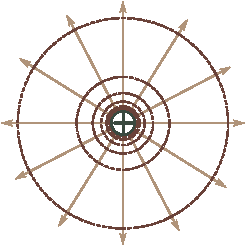
\includegraphics[scale=1]{figures/ch_01/fig_1_8.pdf}
			\caption[]{}
			\label{fig:1_8}
		\end{center}
	\end{minipage}
	\hspace{-0.05cm}
	\begin{minipage}[t]{0.5\linewidth}
		\begin{center}
			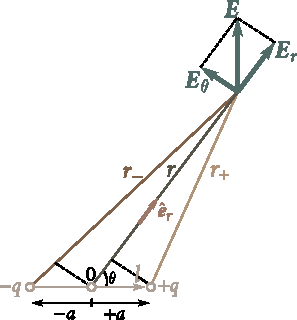
\includegraphics[scale=0.95]{figures/ch_01/fig_1_9.pdf}
			\caption[]{}
			\label{fig:1_9}
		\end{center}
	\end{minipage}
\vspace{-0.4cm}
\end{figure}

Equipotential surfaces for a homogeneous field are a collection of equispaced planes at right angles to the direction of the field.

\section{Dipole}\label{sec:1_9}

An \textbf{electric dipole} is defined as a system of two point charges $+q$ and $-q$ identical in value and opposite in sign, the distance between which is much smaller than that to the points at which the field of the system is being determined. The straight line passing through both charges is called the \textbf{dipole axis}.

Let us first calculate the potential and then the field strength of a dipole. This field has axial symmetry. Therefore, the pattern of the field in any plane passing through the dipole axis will be the same, the vector $\vec{E}$ being in this plane. The position of a point relative to the dipole will be characterized with the aid of the position vector $\vec{r}$ or with the aid of the polar coordinates $r$ and $\theta$ (\fig{1_9}). We shall introduce the vector $\vec{l}$ passing from the negative charge to the positive one. The position of the charge $+q$ relative to the centre of the dipole is determined by the vector $\vec{a}$, and of the charge $-q$ by the vector $-\vec{a}$. It is obvious that $\vec{l}=2\vec{a}$. We shall designate the distances to a given point from the charges $+q$ and $-q$ by $r_+$ and $r_-$, respectively.

Owing to the smallness of $a$ in comparison with $r$, we can assume approximately that
\begin{equation}\label{eq:1_47}
\begin{split}
	r_+ &= r - a\cos\theta = r - \vec{a}\!\vec{\cdot}\!\vecuni{r},\\
	r_- &= r + a\cos\theta = r + \vec{a}\!\vec{\cdot}\!\vecuni{r}.
\end{split}
\end{equation}

The potential at a point determined by the position vector $\vec{r}$ is
\begin{equation*}
	\varphi(\vec{r}) = \frac{1}{4\pi\varepsilon_0} \parenthesis{
	\frac{q}{r_+} - \frac{q}{r_-}
	} = \frac{1}{4\pi\varepsilon_0} \frac{q(r_- - r_+)}{r_+ r_-}.
\end{equation*}

\noindent
The product $r_+r_-$ can be replaced with $r^2$. The difference $r_--r_+$ according to Eqs. \eqref{eq:1_47}, is $2(\vec{a}\!\vec{\cdot}\!\vecuni{r})=\vec{l}\!\vec{\cdot}\!\vecuni{r}$. Hence,
\begin{equation}\label{eq:1_48}
	\varphi(\vec{r}) = \frac{1}{4\pi\varepsilon_0} \frac{q(\vec{l}\!\vec{\cdot}\!\vecuni{r})}{r^2} = \frac{1}{4\pi\varepsilon_0} \frac{(\vec{p}\!\vec{\cdot}\!\vecuni{r})}{r^2}
\end{equation}

\noindent
where
\begin{equation}\label{eq:1_49}
	\vec{p} = q\vec{l}
\end{equation}

\noindent
is a characteristic of a dipole called its \textbf{electric moment}. The vector $\vec{p}$ is directed along the dipole axis from the negative charge to the positive one (\fig{1_10}).

\begin{figure}[t]
	\begin{center}
		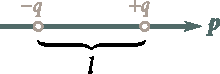
\includegraphics[scale=1.1]{figures/ch_01/fig_1_10.pdf}
		\caption[]{}
		\label{fig:1_10}
	\end{center}
	\vspace{-0.8cm}
\end{figure}

A glance at \eqn{1_48} shows that the field of a dipole is determined by its electric moment $\vec{p}$. We shall see below that the behaviour of a dipole in an external electric field is also determined by its electric moment $\vec{p}$. A comparison with \eqn{1_26} shows that the potential of a dipole field diminishes with the distance more rapidly (as $1/r^2$) than the potential of a point charge field (which changes in proportion to $1/r$).

It can be seen from \fig{1_9} that $\vec{p}\!\vec{\cdot}\!\vecuni{r}=p\cos\theta$. Therefore, \eqn{1_48} can be written as follows:
\begin{equation}\label{eq:1_50}
	\varphi(r,\theta) = \frac{1}{4\pi\varepsilon_0} \frac{p\cos\theta}{r^2}.
\end{equation}

To find the field strength of a dipole, let us calculate the projections of the vector $\vec{E}$ onto two mutually perpendicular directions by \eqn{1_44}. One of them is determined by the motion of a point due to the change in the distance $r$ (with $\theta$ fixed), the other by the motion of the point due to the change in the angle $\theta$ (with $r$ fixed, see \fig{1_9}). The first projection is obtained by differentiation of \eqn{1_50} with respect to $r$:
\begin{equation}\label{eq:1_51}
	E_r = - \diffpartial{\varphi}{r} = \frac{1}{4\pi\varepsilon_0} \frac{2p\cos\theta}{r^3}.
\end{equation}

\noindent
We shall find the second projection (let us designate it by $E_{\theta}$) by taking the ratio of the increment of the potential $\varphi$ obtained when the angle $\theta$ grows by $\deriv{\theta}$ to the distance $r\,\deriv{\theta}$ over which the end of the segment $r$ moves (in this case the quantity $\deriv{l}$ in \eqn{1_44} equals $r\,\deriv{\theta}$]. Thus,
\begin{equation*}
	E_{\theta} = - \frac{1}{r}\diffpartial{\varphi}{\theta}.
\end{equation*}

\noindent
Introducing the value of the derivative of function \eqref{eq:1_50} with respect to $\theta$ we get
\begin{equation}\label{eq:1_52}
	E_{\theta} = \frac{1}{4\pi\varepsilon_0} \frac{p\sin\theta}{r^3}.
\end{equation}

\noindent
The sum of the squares of Eqs. \eqref{eq:1_51} and \eqref{eq:1_52} gives the square of the vector $\vec{E}$ (see \fig{1_9}):
\begin{align*}
	E^2 &= E_r^2 + E_{\theta}^2 = \parenthesis{\frac{1}{4\pi\varepsilon_0}}^2 \parenthesis{\frac{p}{r^3}}^2 \parenthesis{4\cos^2\theta + \sin^2\theta}\\
		&= \parenthesis{\frac{1}{4\pi\varepsilon_0}}^2 \parenthesis{\frac{p}{r^3}}^2 \parenthesis{1 + 3\cos^2\theta}.
\end{align*}

\noindent
Hence
\begin{equation}\label{eq:1_53}
	E = \frac{1}{4\pi\varepsilon_0} \frac{p}{r^3} \parenthesis{1 + 3\cos^2\theta}^{1/2}.
\end{equation}

Assuming in \eqn{1_53} that $\theta=0$, we get the strength on the dipole axis:
\begin{equation}\label{eq:1_54}
	E_{\parallel} = \frac{1}{4\pi\varepsilon_0} \frac{2p}{r^3}.
\end{equation}

\noindent
The vector $\vec{E}_{\parallel}$ is directed along the dipole axis. This is in agreement with the axial symmetry of the problem. Examination of \eqn{1_51} shows that $E_r>0$ when $\theta=0$, and $E_r<0$ when $\theta=\pi$. This signifies that in any case the vector $\vec{E}_{\parallel}$ has a direction coinciding with that from $-q$ to $+q$ (\ie, with the direction of $\vec{p}$). Equation \eqref{eq:1_54} can therefore be written in the vector form:
\begin{equation}\label{eq:1_55}
	\vec{E}_{\parallel} = \frac{1}{4\pi\varepsilon_0} \frac{2\vec{p}}{r^3}.
\end{equation}

Assuming in \eqn{1_53} that $\theta=\pi/2$, we get the field strength on the straight line passing through the centre of the dipole and perpendicular to its axis:
\begin{equation}\label{eq:1_56}
	E_{\perp} = \frac{1}{4\pi\varepsilon_0} \frac{p}{r^3}.
\end{equation}

\noindent
By \eqn{1_51}, when $\theta=\pi/2$, the projection $E_r$ equals zero. Hence, the vector $\vec{E}_{\perp}$ is parallel to the dipole axis. It follows from \eqn{1_52} that when $\theta=\pi/2$, the projection $E_{\theta}$ is positive. This signifies that the vector $\vec{E}_{\perp}$ is directed toward the growth of the angle $\theta$, \ie, antiparallel to the vector $\vec{p}$.

The field strength of a dipole is characterized by the circumstance that it diminishes with the distance from the dipole in proportion to $1/r^3$, \ie, more rapidly than the field strength of a point charge (which diminishes in proportion to $1/r^2$).

\begin{figure}[t]
	\begin{minipage}[t]{0.5\linewidth}
		\begin{center}
			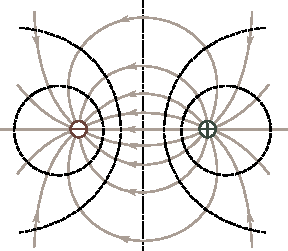
\includegraphics[scale=1]{figures/ch_01/fig_1_11.pdf}
			\caption[]{}
			\label{fig:1_11}
		\end{center}
	\end{minipage}
	\hspace{-0.05cm}
	\begin{minipage}[t]{0.5\linewidth}
		\begin{center}
			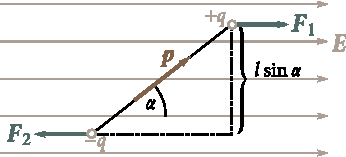
\includegraphics[scale=1]{figures/ch_01/fig_1_12.pdf}
			\caption[]{}
			\label{fig:1_12}
		\end{center}
	\end{minipage}
\vspace{-0.4cm}
\end{figure}

Figure \ref{fig:1_11} shows $\vec{E}$ lines (the solid lines) and equipotential surfaces (the dash lines) of the field of a dipole. According to \eqn{1_50}, when $\theta=\pi/2$, the potential vanishes for all the $r$'s. Thus, all the points of a plane at right angles to the dipole axis and passing through its middle have a zero potential. This could have been predicted because the distances from the charges $+q$ and $-q$ to any point of this plane are identical.

Now let us turn to the behaviour of a dipole in an external electric field. If a dipole is placed in a homogeneous electric field, the charges $+q$ and $-q$ forming the dipole will be under the action of the forces $\vec{F}_1$ and $\vec{F}_2$ equal in magnitude, but opposite in direction (\fig{1_12}). These forces form a couple whose arm is $l\sin\alpha$, \ie, depends on the orientation of the dipole relative to the field. The magnitude of each of the forces is $qE$. Multiplying it by the arm, we get the magnitude of the torque acting on a dipole:
\begin{equation}\label{eq:1_57}
	T = q E l \sin\alpha = p E \sin\alpha
\end{equation}

\noindent
($p$ is the electric moment of the dipole). It is easy to see that \eqn{1_57} can be written in the vector form
\begin{equation}\label{eq:1_58}
	\vec{T} = \vecprod{p}{E}.
\end{equation}

\noindent
The torque \eqref{eq:1_58} tends to turn a dipole so that its electric moment $\vec{p}$ is in the direction of the field.

Let us find the potential energy belonging to a dipole in an external electric field. By \eqn{1_29}, this energy is
\begin{equation}\label{eq:1_59}
	\ab{W}{p} = q\varphi_+ - q\varphi_- = q(\varphi_+ - \varphi_-).
\end{equation}

\noindent
Here $\varphi_+$ and $\varphi_-$ are the values of the potential of the external field at the points where the charges $+q$ and $-q$ are placed.

The potential of a homogeneous field diminishes linearly in the direction of the vector $\vec{E}$. Assuming that the $x$-axis is this direction (\fig{1_13}), we can write that $E=E_x=-\diffin{\varphi}{x}$. A glance at \fig{1_13} shows that the difference $\varphi_+-\varphi_-$ equals the increment of the potential on the segment $\Delta{x}=l\cos\alpha$:
\begin{equation*}
	\varphi_+ - \varphi_- = \diff{\varphi}{x} l\cos\alpha = -El\cos\alpha.
\end{equation*}

\begin{figure}[t]
	\begin{minipage}[t]{0.5\linewidth}
		\begin{center}
			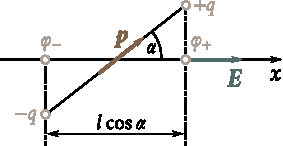
\includegraphics[scale=1]{figures/ch_01/fig_1_13.pdf}
			\caption[]{}
			\label{fig:1_13}
		\end{center}
	\end{minipage}
	\hspace{-0.05cm}
	\begin{minipage}[t]{0.5\linewidth}
		\begin{center}
			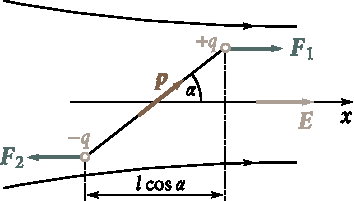
\includegraphics[scale=1]{figures/ch_01/fig_1_14.pdf}
			\caption[]{}
			\label{fig:1_14}
		\end{center}
	\end{minipage}
\vspace{-0.4cm}
\end{figure}

\noindent
Introducing this value into \eqn{1_59}, we find that
\begin{equation}\label{eq:1_60}
	\ab{W}{p} = - q E l \cos\alpha = - p E \cos\alpha.
\end{equation}

\noindent
Here $\alpha$ is the angle between the vectors $\vec{p}$ and $\vec{E}$. We can therefore write \eqn{1_60} in the form
\begin{equation}\label{eq:1_61}
	\ab{W}{p} = - \vecdot{p}{E}.
\end{equation}

\noindent
We must note that this expression takes no account of the energy of interaction of the charges $+q$ and $-q$ forming a dipole.

We have obtained \eqn{1_61} assuming for simplicity's sake that the field is homogeneous. This equation also holds, however, for an inhomogeneous field.

Let us consider a dipole in an inhomogeneous field that is symmetrical relative to the $x$-axis\footnote{A particular case of such a field is that of a point charge if we take a straight line passing through the charge as the $x$-axis.}. Let the centre of the dipole be on this axis, the dipole electric moment making with the axis an angle $\alpha$, differing from $\pi/2$ (\fig{1_14}). In this case, the forces acting on the dipole charges are not identical in magnitude. Therefore, apart from
the rotational moment (torque), the dipole will experience a force tending to move it in the direction of the $x$-axis. To find the value of this force, we shall use \eqn{1_40}, according to which
\begin{equation*}
	F_x = -\diffpartial{\ab{W}{p}}{x},\quad F_y = -\diffpartial{\ab{W}{p}}{y},\quad F_z = -\diffpartial{\ab{W}{p}}{z}.
\end{equation*}

\noindent
In view of \eqn{1_60}, we can written
\begin{equation*}
	\ab{W}{p}(x,y,z) = -p E(x,y,z)\cos\alpha
\end{equation*}

\noindent
(we consider the orientation of the dipole relative to the vector $\vec{E}$ to be constant, $\alpha=\text{constant}$).

For points on the $x$-axis, the derivatives of $E$ with respect to $y$ and $z$ are zero. Accordingly, $\diffinpartial{\ab{W}{p}}{y}=\diffinpartial{\ab{W}{p}}{z}=0$. Thus, only
the force component $F_x$ differs from zero. It is
\begin{equation}\label{eq:1_62}
	F_x = - \diffpartial{\ab{W}{p}}{x} = p \diffpartial{E}{x} \cos\alpha.
\end{equation}

\noindent
This result can be obtained if we take account of the fact that the field strength at the points where the charges $+q$ and $-q$ are (see
\fig{1_14}) differs by the amount $(\diffinpartial{E}{x})l\cos\alpha$. Accordingly, the difference between the forces acting on the charges is $q(\diffinpartial{E}{x})l\cos\alpha$, which coincides with \eqn{1_62}.

When $\alpha$ is less than $\pi/2$, the value of $F_x$ determined by \eqn{1_62} is positive. This signifies that under the action of the force the dipole is pulled into the region of a stronger field (see \fig{1_14}). When $\alpha$ is greater than $\pi/2$, the dipole is pushed out of the field.

\begin{figure}[t]
	\begin{center}
		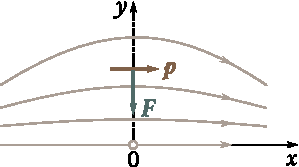
\includegraphics[scale=1]{figures/ch_01/fig_1_15.pdf}
		\caption[]{}
		\label{fig:1_15}
	\end{center}
	\vspace{-0.8cm}
\end{figure}

In the case shown in \fig{1_15}, only the derivative $\diffinpartial{E}{y}$ differs from zero for points on the $y$-axis. Therefore, the force acting on the dipole is determined by the component
\begin{equation*}
	F_y = -\diffpartial{\ab{W}{p}}{y} = p \diffpartial{E}{y},\quad (\cos\alpha=1).
\end{equation*}

\noindent
The derivative $\diffinpartial{E}{y}$ is negative. Consequently, the force is directed as shown in the figure. Thus, in this case too, the dipole is pulled into the field.

We shall note that like $-\diffinpartial{\ab{W}{p}}{x}$ gives the projection of the force acting on the system onto the $x$-axis, so does the derivative of \eqn{1_60} with respect to $\alpha$ taken with the opposite sign give the projection of the torque onto the $\alpha$-``axis'': $T_{\alpha}=-pE\sin\alpha$. The minus sign was obtained because the $\alpha$-``axis'' and the torque $T$ are directed oppositely (see \fig{1_12}).

\section{Field of a System of Charges at Great Distances}\label{sec:1_10}

Let us take a system of $N$ charges $q_1, q_2, \ldots, q_N$ in a volume having linear dimensions of the order of $l$, and study the field set up by this system at distances $r$ that are great in comparison with $l$ ($r>l$). We take the origin of coordinates $0$ inside the volume occupied by the system and shall determine the positions of the charges with the aid of the position vectors $\vec{r}_i$, (\fig{1_16}; to simplify the figure, we have shown only the position vector of the $i$-th charge).

\begin{figure}[t]
	\begin{center}
		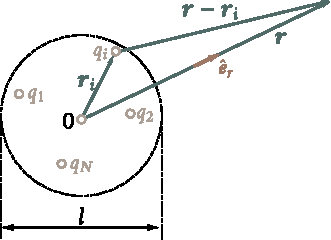
\includegraphics[scale=0.95]{figures/ch_01/fig_1_16.pdf}
		\caption[]{}
		\label{fig:1_16}
	\end{center}
	\vspace{-1.0cm}
\end{figure}

The potential at the point determined by the position vector $\vec{r}$ is
\begin{equation}\label{eq:1_63}
	\varphi(\vec{r}) = \frac{1}{4\pi\varepsilon_0} \sum_{i=1}^N \frac{q_i}{\absolute{\vec{r} - \vec{r}_i}}.
\end{equation}

\noindent
Owing to the smallness of $r_i$ in comparison with $r$, we can assume that
\begin{equation*}
	\absolute{\vec{r} - \vec{r}_i} = r - \vec{r}_i\!\vec{\cdot}\!\vecuni{r} = r\parenthesis{1 - \frac{\vec{r}_i\!\vec{\cdot}\!\vecuni{r}}{r}}
\end{equation*}

\noindent
[compare with Eqs. \eqref{eq:1_47}]. Introduction of this expression into
\eqn{1_63} yields
\begin{equation}\label{eq:1_64}
	\varphi(\vec{r}) = \frac{1}{4\pi\varepsilon_0} \sum_{i=1}^N \frac{q_i}{r} \bracket{\frac{1}{1 - \parenthesis{\vec{r}_i\!\vec{\cdot}\!\vecuni{r}/r}}}.
\end{equation}

\noindent
Using the formula
\begin{equation*}
	\frac{1}{1-x} \approx 1 + x
\end{equation*}

\noindent
which holds when $x\ll 1$, we can transform \eqn{1_64} as follows:
\begin{align}
	\varphi(\vec{r}) &= \frac{1}{4\pi\varepsilon_0} \sum_{i=1}^N \frac{q_i}{r} \parenthesis{1 + \frac{\vec{r}_i\!\vec{\cdot}\!\vecuni{r}}{r}}\nonumber\\
	&= \frac{1}{4\pi\varepsilon_0} \frac{1}{r} \sum_{i=1}^N q_i + \frac{1}{4\pi\varepsilon_0} \frac{1}{r^2} \parenthesis{\sum_{i=1}^N q_i \vec{r}_i}\!\vec{\cdot}\!\vecuni{r}. \label{eq:1_65}
\end{align}

\noindent
The first term of the expression obtained is the potential of the field of a point charge having the value $q=\sum_iq_i$ [compare with \eqn{1_26}]. The second term has the same form as the expression determining the potential of a dipole field, the part of the electric moment of the dipole being played by the quantity
\begin{equation}\label{eq:1_66}
	\vec{p} = \sum_{i=1}^N q_i \vec{r}_i.
\end{equation}

\noindent
This quantity is called the \textbf{dipole electric moment} of a system of charges. It is easy to verify that for a dipole \eqn{1_66} transforms
into the expression $\vec{p}=q\vec{l}$ which we are already familiar with.

\begin{figure}[t]
	\begin{minipage}[t]{0.4\linewidth}
		\begin{center}
			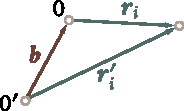
\includegraphics[scale=1]{figures/ch_01/fig_1_17.pdf}
			\caption[]{}
			\label{fig:1_17}
		\end{center}
	\end{minipage}
	\hspace{-0.05cm}
	\begin{minipage}[t]{0.6\linewidth}
		\begin{center}
			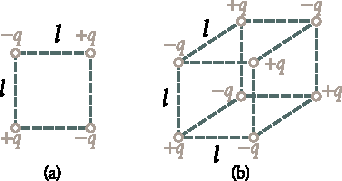
\includegraphics[scale=1]{figures/ch_01/fig_1_18.pdf}
			\caption[]{}
			\label{fig:1_18}
		\end{center}
	\end{minipage}
\vspace{-0.4cm}
\end{figure}

If the total charge of a system is zero ($\sum_iq_i=0$), the value of the dipole moment does not depend on our choice of the origin of coordinates. To convince ourselves that this is true, let us take two arbitrary origins of coordinates $0$ and $0'$ (\fig{1_17}). The position vectors of the $i$-th charge conducted from these points are related as follows:
\begin{equation}\label{eq:1_67}
	\vec{r}_i' = \vec{b} + \vec{r}_i
\end{equation}

\noindent
(what the vector $\vec{b}$ is clear from the figure). With account taken of \eqn{1_67}, the dipole moment in the system with the origin $0'$ is
\begin{equation*}
	\vec{p}' = \sum_i q_i \vec{r}_i = \sum_i q_i (\vec{b} + \vec{r}_i) = \vec{b} \sum_i q_i + \sum_i q_i \vec{r}_i.
\end{equation*}

\noindent
The first addend equals zero (because $\sum_iq_i=0$). The second one is $\vec{p}$---the dipole moment in a coordinate system with its origin at $0$. We have thus obtained that $\vec{p}'=\vec{p}$.

Equation \eqref{eq:1_65} is in essence the first two terms of the series expansion of function \eqref{eq:1_63} by powers of $r_i/r$. When $\sum_iq_i\neq 0$, the first term of \eqn{1_65} makes the main contribution to the potential (the second term diminishes in proportion to $1/r^2$ and is therefore much smaller than the first one). For an electrically neutral system ($\sum_iq_i=0$), the first term equals zero, and the potential is determined mainly by the second term of \eqn{1_65}. This is how matters stand, in particular, for the field of a dipole.

For the system of charges depicted in \fig{1_18}a and called a \textbf{quadrupole}, both $\sum_iq_i$ and $\vec{p}$ equal zero so that \eqn{1_65} gives a zero value of the potential. Actually, however, the field of a quadrupole, although it is much weaker than that of a dipole (with the same values of $q$ and $l$), differs from zero. The potential of the field set up by a quadrupole is determined mainly by the third term of the expansion that is proportional to $1/r^3$. To obtain this term, we must take into consideration quantities of the order of $(r_i/r)^2$ which we disregarded in deriving \eqn{1_65}. For the system of charges shown in \fig{1_18}b and called an \textbf{octupole}, the third term of the expansion also equals zero. The potential of the field of such a system is determined by the fourth term of the expansion, which is proportional to $1/r^4$.

It must be noted that the quantity equal to $\sum_iq_i$ in the numerator of the first term of \eqn{1_65} is called a \textbf{monopole} or a \textbf{zero-order multipole}, a dipole is also called a \textbf{first-order multipole}, a quadrupole is called a \textbf{second-order multipole}, and so on.

Thus, in the general case, the field of a system of charges at great distances can be represented as the superposition of fields set up by multipoles of different orders---a monopole, dipole, quadrupole, octupole, etc.

\section{A Description of the Properties of Vector Fields}\label{sec:1_11}

To continue our study of the electric field, we must acquaint ourselves with the mathematical tools used to describe the properties of vector fields. These tools are called \textbf{vector analysis}. In the present section, we shall treat the fundamental concepts and selected formulas of vector analysis, and also prove its two main theorems---the Ostrogradsky-Gauss theorem (sometimes called Gauss's divergence theorem) and Stokes's theorem.

The quantities used in vector analysis can be best illustrated for the field of the velocity vector of a flowing liquid. We shall therefore introduce these quantities while dealing with the flow of an ideal incompressible liquid, and then extend the results obtained to vector fields of any nature.

We are already acquainted with one of the concepts of vector analysis. This is the \textbf{gradient}, used to characterize scalar fields. If the value of the scalar quantity $\varphi=\varphi(x, y, z)$ is compared with every point P having the coordinates $x, y, z$, we say that the scalar field of $\varphi$ has been set. The gradient of the quantity $\varphi$ is defined as the vector
\begin{equation}\label{eq:1_68}
	\grad{\varphi} = \diffpartial{\varphi}{x}\,\vecuni{x} + \diffpartial{\varphi}{y}\,\vecuni{y} + \diffpartial{\varphi}{z}\,\vecuni{z}.
\end{equation}

The increment of the function $\varphi$ upon displacement over the length $\deriv{\vec{l}}=\vecuni{x}\,\deriv{x}+\vecuni{y}\,\deriv{y}+\vecuni{z}\,\deriv{z}$ is
\begin{equation*}
	\deriv{\varphi} = \diffpartial{\varphi}{x}\,\deriv{x} + \diffpartial{\varphi}{y}\,\deriv{y} + \diffpartial{\varphi}{z}\,\deriv{z}
\end{equation*}

\noindent
which can be written in the form
\begin{equation}\label{eq:1_69}
	\deriv{\varphi} = \grad{\varphi} \ccdot \deriv{\vec{l}}.
\end{equation}

Now we shall go over to establishing the characteristics of vector fields.

\begin{figure}[t]
	\begin{center}
		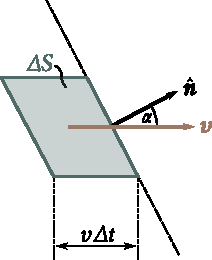
\includegraphics[scale=1]{figures/ch_01/fig_1_19.pdf}
		\caption[]{}
		\label{fig:1_19}
	\end{center}
	\vspace{-0.8cm}
\end{figure}

\textbf{Vector flux.} Assume that the flow of a liquid is characterized by the field of the velocity vector. The volume of liquid flowing in unit time through an imaginary surface $S$ is called the flux of the liquid through this surface. To find the flux, let us divide the surface into elementary sections of the size $\Delta{S}$. It can be seen from \fig{1_19} that during the time $\Delta{t}$ a volume of liquid equal to
\begin{equation*}
	\Delta{V} = (\Delta{S}\cos\alpha) v\Delta{t}
\end{equation*}

\noindent
will pass through section $\Delta{S}$. Dividing this volume by the time $\Delta{t}$, we shall find the flux through surface $\Delta{S}$:
\begin{equation*}
	\Delta{\Phi} = \frac{\Delta{V}}{\Delta{t}} = \Delta{S} v \cos\alpha.
\end{equation*}

\noindent
Passing over to differentials, we find that
\begin{equation}\label{eq:1_70}
	\deriv{\Phi} = (v \cos\alpha)\, \deriv{S}.
\end{equation}

\noindent
Equation \eqref{eq:1_70} can be written in two other ways. First, if we take into account that $v\cos\alpha$ gives the projection of the velocity vector onto the normal $\vecuni{n}$ to area $\deriv{S}$, we can write \eqn{1_70} in the form
\begin{equation}\label{eq:1_71}
	\deriv{\Phi} = v_n\, \deriv{S}.
\end{equation}

\noindent
Second, we can introduce the vector $\deriv{\vec{S}}$ whose magnitude equals that of area $\deriv{S}$, while its direction coincides with the direction of a normal $\hatvec{n}$ to the area:
\begin{equation*}
	\deriv{\vec{S}} = \deriv{S}\, \hatvec{n}.
\end{equation*}

\noindent
Since the direction of the vector $\hatvec{n}$ is chosen arbitrarily (it can be directed to either side of the area), then $\deriv{\vec{S}}$ is not a true vector, but is a pseudo vector. The angle $\alpha$ in \eqn{1_70} is the angle between the vectors $\vec{v}$ and $\deriv{\vec{S}}$. Hence, this equation can be written in the form
\begin{equation}\label{eq:1_72}
	\deriv{\Phi} = \vec{v} \ccdot \deriv{\vec{S}}.
\end{equation}

By summating the fluxes through all the elementary areas into which we have divided surface $S$, we get the flux of the liquid through $S$:
\begin{equation}\label{eq:1_73}
	\Phi_v = \int_S \vec{v} \ccdot \deriv{\vec{S}} = \int_S v_n\, \deriv{S}.
\end{equation}

\noindent
A similar expression written for an arbitrary vector field $\vec{a}$, \ie, the quantity
\begin{equation}\label{eq:1_74}
	\Phi_a = \int_S \vec{a} \ccdot \deriv{\vec{S}} = \int_S a_n\, \deriv{S}
\end{equation}

\noindent
is called the \textbf{flux of the vector a through surface} $S$. In accordance with this definition, the flux of a liquid can be called the flux of the vector $\vec{v}$ through the relevant surface [see \eqn{1_73}].

The flux of a vector is an algebraic quantity. Its sign depends on the choice of the direction of a normal to the elementary areas into which surface $S$ is divided in calculating the flux. Reversal of the direction of the normal changes the sign of $a_n$ and, therefore, the sign of the quantity \eqref{eq:1_74}. The customary practice for closed surfaces is calculation of the flux ``emerging outward'' from the region enclosed by the surface. Accordingly, in the following we shall always implicate that $\hatvec{v}$ is an outward normal.

\begin{figure}[t]
	\begin{center}
		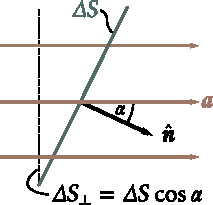
\includegraphics[scale=0.95]{figures/ch_01/fig_1_20.pdf}
		\caption[]{}
		\label{fig:1_20}
	\end{center}
	\vspace{-1.0cm}
\end{figure}

We can give an illustrative geometrical interpretation of the vector flux. For this purpose, we shall represent a vector field by a system of
lines $\vec{a}$ constructed so that the density of the lines at every point is numerically equal to the magnitude of the vector $\vec{a}$ at the same point of the field (compare with the rule for constructing the lines of the vector $\vec{E}$ set out at the end of \sect{1_5}). Let us find the number $\Delta{N}$ of intersections of the field lines with the imaginary area $\Delta{S}$. A glance at \fig{1_20} shows that this number equals the density of the lines (\ie, $a$) multiplied by $\Delta{S}_{\perp}=\Delta{S}\cos\alpha$:
\begin{equation*}
	\Delta{N}\, (=)\, a \Delta{S}\cos\alpha = a_n \Delta{S}.
\end{equation*}

\noindent
We are speaking only about the numerical equality between $\Delta{N}$ and $a_n\Delta{S}$. This is why the equality sign is confined in parentheses. According to \eqn{1_74}, the expression $a_n\Delta{S}$ is $\Delta{\Phi}$---the flux of the vector a through area $\Delta{S}$. Thus,
\begin{equation}\label{eq:1_75}
	\Delta{N}\, (=)\, \Delta{\Phi}_a.
\end{equation}

For the sign of $\Delta{N}$ to coincide with that of $\Delta{\Phi}_a$, we must consider those intersections to be positive for which the angle $\alpha$ between the positive direction of a field line and a normal to the area is acute. The intersection should be considered negative if the angle $\alpha$ is obtuse. For the area shown in \fig{1_20}, all three intersections are positive: $\Delta{N}=+3$ ($\Delta{\Phi}_a$ in this case is also positive because $a_n>0$). If the direction of the normal in \fig{1_20} is reversed, the intersections will become negative ($\Delta{N}=-3$), and the flux $\Delta{\Phi}_a$ will also be negative.

Summation of \eqn{1_75} over the finite imaginary surface $S$ yields
\begin{equation}\label{eq:1_76}
	\Delta{\Phi}_a\, (=)\, \sum\Delta{N} = N_+ - N_-
\end{equation}

\noindent
where $N_+$ and $N_-$ are the total number of positive and negative intersections of the field lines with surface $S$, respectively.

The reader may be puzzled by the circumstance that since the flux, as a rule, is expressed by a fractional number, the number of intersections of the field lines with a surface compared with the flux will also be fractional. Do not be confused by this, however. Field lines are a purely conditional image deprived of a physical meaning.

Let us take an imaginary surface in the form of a strip of paper whose bottom part is twisted relative to the top one through the angle $\pi$ (\fig{1_21}). The direction of a normal must be chosen identically for the entire surface. Hence, if in the top part of the strip a positive normal is directed to the right, then in the bottom part a normal will be directed to the left. Accordingly, the intersections of the field lines depicted in \fig{1_21} with the top half of the surface must be considered positive, and with the bottom half, negative.

\begin{figure}[t]
	\begin{minipage}[t]{0.4\linewidth}
		\begin{center}
			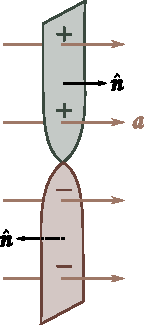
\includegraphics[scale=0.95]{figures/ch_01/fig_1_21.pdf}
			\caption[]{}
			\label{fig:1_21}
		\end{center}
	\end{minipage}
	\hspace{-0.05cm}
	\begin{minipage}[t]{0.6\linewidth}
		\begin{center}
			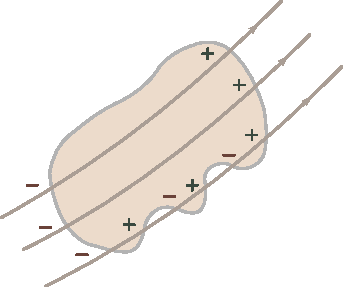
\includegraphics[scale=0.95]{figures/ch_01/fig_1_22.pdf}
			\caption[]{}
			\label{fig:1_22}
		\end{center}
	\end{minipage}
\vspace{-0.4cm}
\end{figure}

An outward normal is considered to be positive for a closed surface (\fig{1_22}). Therefore, the intersections corresponding to outward protrusion of the lines (in this case the angle $\alpha$ is acute) must be taken with the plus sign, and the ones appearing when the lines enter the surface (in this case the angle $\alpha$ is obtuse) must be taken with the minus sign.

Inspection of \fig{1_22} shows that when the field lines enter a closed surface continuously, each line when intersecting the surface enters it and emerges from it the same number of times. As a result, the flux of the corresponding vector through this surface equals zero. It is easy to see that if field lines end inside a surface, the vector flux through the closed surface will numerically equal the difference between the number of lines beginning inside the surface ($\ab{N}{beg}$) and the number of lines terminating inside the surface ($\ab{N}{term}$):
\begin{equation}\label{eq:1_77}
	\Phi_a\, (=)\, \ab{N}{beg} - \ab{N}{term}.
\end{equation}

\noindent
The sign of the flux depends on which of these numbers is greater. When $\ab{N}{beg}$ is equal to $\ab{N}{term}$, the flux equals zero.

\textbf{Divergence.} Assume that we are given the field of the velocity vector of an incompressible continuous liquid. Let us take an imaginary closed surface $S$ in the vicinity of point P (\fig{1_23}). If in the volume confined by this surface no liquid appears and no liquid vanishes, then the flux flowing outward through the surface will evidently equal zero. A liquid flux $\Phi_v$ other than zero will indicate that there are liquid sources or sinks inside the surface, \ie, points at which the liquid enters the volume (sources) or emerges from it (sinks). The magnitude of the flux determines the total algebraic power of the sources and sinks\footnote{The power of a source (sink) is defined as the volume of liquid discharged (absorbed) in unit time. A sink can be considered as a source with a negative power.}. When the sources predominate over the sinks, the magnitude of the flux will be positive, and when the sinks predominate, negative.

\begin{figure}[t]
	\begin{center}
		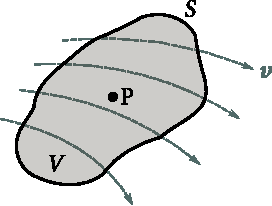
\includegraphics[scale=1]{figures/ch_01/fig_1_23.pdf}
		\caption[]{}
		\label{fig:1_23}
	\end{center}
	\vspace{-0.8cm}
\end{figure}

The quotient obtained when dividing the flux $\Phi_v$ by the volume which it flows out from, \ie,
\begin{equation}\label{eq:1_78}
	\frac{\Phi_v}{V}
\end{equation}

\noindent
gives the average unit power of the sources confined in the volume $V$. In the limit when $V$ tends to zero, \ie, when the volume $V$ contracts to point P, expression \eqref{eq:1_78} gives the true unit power of the sources at point P, which is called the \textbf{divergence} of the vector $\vec{v}$ (it is designated by $\diverg{\vec{v}}$). Thus, by definition,
\begin{equation*}
	\diverg{\vec{v}} = \lim_{V\to \text{P}} \frac{\Phi_v}{V}.
\end{equation*}

\noindent
The divergence of any vector $\vec{a}$ is determined in a similar way:
\begin{equation}\label{eq:1_79}
	\diverg{\vec{a}} = \lim_{V\to \text{P}} \frac{\Phi_v}{V} = \lim_{V\to \text{P}} \oint \vec{a} \ccdot \deriv{\vec{S}}.
\end{equation}

\noindent
The integral is taken over arbitrary closed surface $S$ surrounding point P\footnote{The circle on the integral sign signifies that integration is performed over a closed surface.}; $V$ is the volume confined by this surface. Since the transition $V\to$P is being performed upon which $S$ tends to zero, we can assume that \eqn{1_79} cannot depend on the shape of the surface. This assumption is confirmed by strict calculations.

Let us surround point P with a spherical surface of an extremely small radius $r$ (\fig{1_24}). Owing to the smallness of $r$, the volume $V$ enclosed by the sphere will also be very small. We can therefore consider with a high degree of accuracy that the value of $\diverg{\vec{a}}$ within the limits of the volume $V$ is constant\footnote{It is assumed that the value of $\diverg{\vec{a}}$ changes continuously, without any jumps, when passing from one point of a field to another.}. In this case, we can write in accordance with \eqn{1_79} that
\begin{equation*}
	\Phi_a \approx (\diverg{\vec{a}}) V
\end{equation*}

\noindent
where $\Phi_a$ is the flux of the vector a through the surface surrounding the volume $V$. By \eqn{1_77}, $\Phi_a$ equals $\ab{N}{beg}$, the number of lines of a beginning inside $V$ if $\diverg{\vec{a}}$ at point P is positive, or $\ab{N}{term}$, the number of lines of a terminating inside $V$ if $\diverg{\vec{a}}$ at point P is negative.

It follows from the above that the lines of the vector $\vec{a}$ begin in the closest vicinity of a point with a positive divergence. The field lines ``diverge'' from this point; the latter is the ``source'' of the field (\fig{1_24}a). On the other hand, in the vicinity of a point with a negative divergence, the lines of the vector $\vec{a}$ terminate. The field lines ``converge'' toward this point; the latter is the ``sink'' of the field (\fig{1_24}b). The greater the absolute value of $\diverg{\vec{a}}$, the bigger is the number of lines that begin or terminate in the vicinity of the given point.

It can be seen from definition \eqref{eq:1_79} that the divergence is a scalar function of the coordinates determining the positions of points in space (briefly---a point function). Definition \eqref{eq:1_79} is the most general one that is independent of the kind of coordinate system used.

\begin{figure}[t]
	\begin{minipage}[t]{0.5\linewidth}
		\begin{center}
			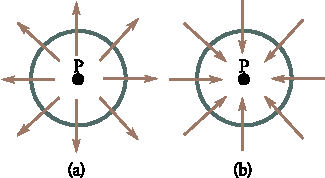
\includegraphics[scale=1.0]{figures/ch_01/fig_1_24.pdf}
			\caption[]{}
			\label{fig:1_24}
		\end{center}
	\end{minipage}
	\hspace{-0.05cm}
	\begin{minipage}[t]{0.5\linewidth}
		\begin{center}
			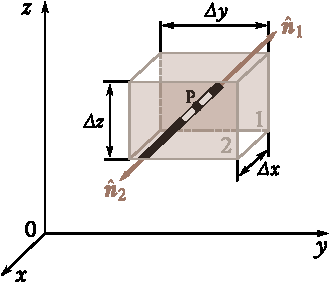
\includegraphics[scale=1.0]{figures/ch_01/fig_1_25.pdf}
			\caption[]{}
			\label{fig:1_25}
		\end{center}
	\end{minipage}
\vspace{-0.4cm}
\end{figure}

Let us find an expression for the divergence in a Cartesian coordinate system. We shall consider a small volume in the form of a parallelepiped with ribs parallel to the coordinate axes in the vicinity of point $P(x, y, z)$ (\fig{1_25}). The vector flux through the surface of the parallelepiped is formed from the fluxes passing through each of the six faces separately.

Let us find the flux through the pair of faces perpendicular to the $x$-axis (in \fig{1_25} these faces are designated by shaded areas and by the numbers 1 and 2). The outward normal $\hatvec{n}_2$ to face 2 coincides with the direction of the $x$-axis. Hence, for points of this face, $a_{n_2}=a_x$. The outward normal $\hatvec{n}_1$ to face 1 is directed oppositely to the $x$-axis. Therefore, for points on this face, $a_{n_2}=-a_x$. The flux through face 2 can be written in the form
\begin{equation*}
	a_{x,2}\Delta{y}\Delta{z}
\end{equation*}

\noindent
where $a_{x,2}$ is the value of $a_x$ averaged over face 2. The flux through face 1 is
\begin{equation*}
	- a_{x,1}\Delta{y}\Delta{z}
\end{equation*}

\noindent
where $a_{x,1}$ is the average value of $a_x$ for face 1. The total flux through faces 1 and 2 is determined by the expression
\begin{equation}\label{eq:1_80}
	(a_{x,2} - a_{x,1}) \Delta{y}\Delta{z}.
\end{equation}

The difference $a_{x,2}-a_{x,1}$ is the increment of the average (over a face) value of $a_x$ upon a displacement along the $x$-axis by $\Delta{x}$. Owing to the smallness of the parallelepiped (we remind our reader that we shall let its dimensions shrink to zero), this increment can be written in the form $(\diffinpartial{a_x}{x})\Delta{x}$, where the value $\diffinpartial{a_x}{x}$ is taken at point P\footnote{The inaccuracy which we tolerate here vanishes when the volume shrinks to point P in the limit transition.}. Therefore, \eqn{1_80} becomes
\begin{equation*}
	\diffpartial{a_x}{x}\Delta{x}\Delta{y}\Delta{z} = \diffpartial{a_x}{x}\Delta{V}.
\end{equation*}

\noindent
Similar reasoning allows us to obtain the following expressions for the fluxes through the pairs of faces perpendicular to the $y$- and $z$-axes:
\begin{equation*}
	\diffpartial{a_y}{y}\Delta{x}\Delta{y}\Delta{z} = \diffpartial{a_y}{y}\Delta{V},\quad \diffpartial{a_z}{z}\Delta{x}\Delta{y}\Delta{z} = \diffpartial{a_z}{z}\Delta{V}.
\end{equation*}

Thus, the total flux through the entire close surface is determined by the expression
\begin{equation*}
	\Phi_a = \parenthesis{\diffpartial{a_x}{x} + \diffpartial{a_y}{y} + \diffpartial{a_z}{z}}\Delta{V}.
\end{equation*}

\noindent
Dividing this expression by $\Delta{V}$, we shall find the divergence of the vector a at point $P(x, y, z)$:
\begin{equation}\label{eq:1_81}
	\diverg{\vec{a}} = \diffpartial{a_x}{x} + \diffpartial{a_y}{y} + \diffpartial{a_z}{z}.
\end{equation}

\textbf{The Ostrogradsky-Gauss Theorem.} If we know the divergence of the vector $\vec{a}$ at every point of space, we can calculate the flux of this vector through any closed surface of finite dimensions. Let us first do this for the flux of the vector $\vec{v}$ (a liquid flux). The product of $\diverg{\vec{v}}$ and $\deriv{V}$ gives the power of the sources of the liquid confined within the volume $\deriv{V}$. The sum of such products, \ie, $\int(\diverg{\vec{v}})\,\deriv{V}$, gives the total algebraic power of the sources confined in the volume $V$ over which integration is performed. Owing to incompressibility of the liquid, the total power of the sources must equal the liquid flux emerging through surface $S$ enclosing the volume $V$. We thus arrive at the equation
\begin{equation*}
	\oint_S \vec{v} \ccdot \deriv{\vec{S}} = \int_V (\diverg{\vec{v}})\,\deriv{V}.
\end{equation*}

\noindent
A similar equation holds for a vector field of any nature:
\begin{equation}\label{eq:1_82}
	\oint_S \vec{a} \ccdot \deriv{\vec{S}} = \int_V (\diverg{\vec{a}})\,\deriv{V}.
\end{equation}

\noindent
This relation is called the \textbf{Ostrogradsky-Gauss} theorem. The integral in the left-hand side of the equation is calculated over an arbitrary closed surface $S$, and the integral in the right-hand side over the volume $V$ enclosed by this surface.

\textbf{Circulation.} Let us revert to the flow of an ideal incompressible liquid. Imagine a closed line---the contour $\Gamma$. Assume that in some way or other we have instantaneously frozen the
liquid in the entire volume except for a very thin closed channel of constant cross section including the contour $\Gamma$ (\fig{1_26}). Depending on the nature of the velocity vector field, the liquid in the channel formed will either be stationary or move along the contour (circulate) in one of the two possible directions. Let us take the quantity equal to the product of the velocity of the liquid in the channel and the length of the contour $l$ as a measure of this motion. This quantity is called the \textbf{circulation} of the vector $\vec{v}$ around the contour $\Gamma$. Thus,
\begin{equation*}
	\text{circulation of $\vec{v}$ around $\Gamma$} = vl
\end{equation*}

\noindent
(since we assumed that the channel has a constant cross section, the magnitude of the velocity, $v$, is a constant).

\begin{figure}[t]
	\begin{center}
		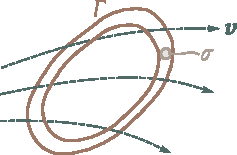
\includegraphics[scale=1]{figures/ch_01/fig_1_26.pdf}
		\caption[]{}
		\label{fig:1_26}
	\end{center}
	\vspace{-0.8cm}
\end{figure}

At the moment when the walls freeze, the velocity component perpendicular to a wall will be eliminated in each of the liquid particles, and only the velocity component tangent to the contour will remain, \ie, $v_l$. The momentum $\deriv{\vec{p}_l}$, is associated with this component. The magnitude of the momentum for a liquid particle contained within a segment of the channel of length $\deriv{l}$ is $\rho\sigma v_l\,\deriv{l}$ ($\rho$ is the density of the liquid, and $\sigma$ is the cross-sectional area of the channel). Since the liquid is ideal, the action of the walls can change only the direction of the vector $\deriv{\vec{p}_l}$, but not its magnitude. The interaction between the liquid particles will cause a redistribution of the momentum between them that will level out the velocities of all the particles. The algebraic sum of the tangential components of the momenta cannot change: the momentum acquired by one of the interacting particles equals the momentum lost by the second particle. This signifies that
\begin{equation*}
	\rho\sigma vl = \oint_{\Gamma} \rho \sigma v_l\,\deriv{l}
\end{equation*}

\noindent
where $v$ is the circulation velocity, and $v_l$ is the tangential component of the liquid's velocity in the volume $\sigma\,\deriv{l}$ at the moment of time preceding the freezing of the channel walls. Cancelling $\rho\sigma$, we get
\begin{equation*}
	\text{circulation of $\vec{v}$ around $\Gamma$} = vl = \oint_{\Gamma} v_l\,\deriv{l}.
\end{equation*}

\noindent
The circulation of any vector $\vec{a}$ around an arbitrary closed contour $\Gamma$ is determined in a similar way:
\begin{equation}\label{eq:1_83}
	\text{circulation of $\vec{a}$ around $\Gamma$} = \oint_{\Gamma} \vec{a} \ccdot \deriv{\vec{l}} = \oint_{\Gamma} a_l\,\deriv{l}.
\end{equation}

It may seem that for the circulation to be other than zero the vector lines must be closed or at least bent in some way or other in the direction of circumventing the contour. It is easy to see that this assumption is wrong. Let us consider the laminar flow of water in a river. The velocity of the water directly at the river bottom is zero and grows as we approach the surface of the water (\fig{1_27}). The streamlines (lines of the vector $\vec{v}$) are straight. Notwithstanding this fact, the circulation of the vector $\vec{v}$ around the contour depicted by the dash line obviously differs from zero. On the other hand, in a field with curved lines, the circulation may equal zero.

\begin{figure}[t]
	\begin{minipage}[t]{0.5\linewidth}
		\begin{center}
			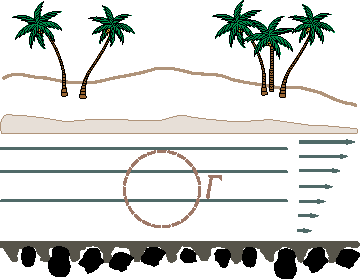
\includegraphics[scale=0.95]{figures/ch_01/fig_1_27.pdf}
			\caption[]{}
			\label{fig:1_27}
		\end{center}
	\end{minipage}
	\hspace{-0.05cm}
	\begin{minipage}[t]{0.5\linewidth}
		\begin{center}
			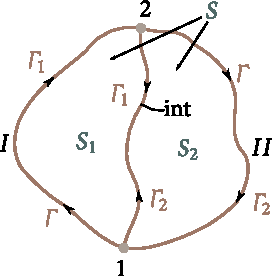
\includegraphics[scale=0.95]{figures/ch_01/fig_1_28.pdf}
			\caption[]{}
			\label{fig:1_28}
		\end{center}
	\end{minipage}
\vspace{-0.6cm}
\end{figure}

Circulation has the property of additivity. This signifies that the sum of the circulations around contours $\Gamma_1$ and $\Gamma_2$ enclosing neighboring surfaces $S_1$ and $S_2$ (\fig{1_28}) equals the circulation around contour $\Gamma$ enclosing surface $S$, which is the sum of surfaces $S_1$ and $S_2$. Indeed, the circulation $C_1$ around the contour bounding surface $S_1$ can be represented as the sum of the integrals
\begin{equation}\label{eq:1_84}
	C_1 = \oint_{\Gamma_1} \vec{a} \ccdot \deriv{\vec{l}} = \int_{1,(I)}^2 \vec{a} \ccdot \deriv{\vec{l}} + \int_{2,(\text{int.})}^1 \vec{a} \ccdot \deriv{\vec{l}}.
\end{equation}

\noindent
The first integral is taken over section $I$ of the outer contour, the second over the interface between surfaces $S_1$ and $S_2$ in direction $2$-$1$.

Similarly, the circulation $C_2$ around the contour enclosing surface $S_2$ is
\begin{equation}\label{eq:1_85}
	C_2 = \oint_{\Gamma_2} \vec{a} \ccdot \deriv{\vec{l}} = \int_{2,(II)}^1 \vec{a} \ccdot \deriv{\vec{l}} + \int_{1,(\text{int.})}^2 \vec{a} \ccdot \deriv{\vec{l}}.
\end{equation}

\noindent
The first integral is taken over section $II$ of the outer contour, the second over the interface between surfaces $S_1$ and $S_2$ in direction $1$-$2$.

The circulation around the contour bounding total surface $S$ can be represented in the form
\begin{equation}\label{eq:1_86}
	C = \oint_{\Gamma} \vec{a} \ccdot \deriv{\vec{l}} = \int_{1,(I)}^2 \vec{a} \ccdot \deriv{\vec{l}} + \int_{2,(II)}^1 \vec{a} \ccdot \deriv{\vec{l}}.
\end{equation}

\noindent
The second addends in Eqs. \eqref{eq:1_84} and \eqref{eq:1_85} differ only in their sign. Therefore, the sum of these expressions will equal \eqn{1_86}. Thus,
\begin{equation}\label{eq:1_87}
	C = C_1 + C_2.
\end{equation}

Equation \eqref{eq:1_87} which we have proved does not depend on the shape of the surfaces and holds for any number of addends. Hence, if we divide an arbitrary open surface $S$ into a great number of elementary surfaces $\Delta{S}$\footnote{In the figure, the elementary surfaces are depicted in the form of rectangles. Actually, their shape may be absolutely arbitrary.} (\fig{1_29}), then the circulation around the contour enclosing $S$ can be written as the sum of the elementary circulations $\Delta{C}$ around the contours enclosing the $\Delta{S}$'s:
\begin{equation}\label{eq:1_88}
	C = \sum_i \Delta{C}_i.
\end{equation}

\begin{figure}[t]
	\begin{center}
		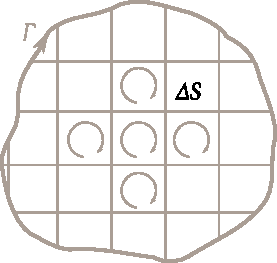
\includegraphics[scale=1]{figures/ch_01/fig_1_29.pdf}
		\caption[]{}
		\label{fig:1_29}
	\end{center}
	\vspace{-0.8cm}
\end{figure}

\textbf{Curl.} The additivity of the circulation permits us to introduce the concept of unit circulation, \ie, consider the ratio of the circulation $C$ to the magnitude of surface $S$ around which the circulation ``flows''. When surface $S$ is finite, the ratio $C/S$ gives the mean value of the unit circulation. This value characterizes the properties of a field averaged over surface $S$. To obtain the characteristic of the field at point P, we must reduce the dimensions of the surface, making it shrink to point P. The ratio $C/S$ tends to a limit that characterizes the properties of the field at point P.

Thus, let us take an imaginary contour $\Gamma$ in a plane passing through point P, and consider the expression
\begin{equation}\label{eq:1_89}
	\lim_{S\to\text{P}} \frac{C_a}{S}
\end{equation}

\noindent
where $C_a$ is the circulation of the vector $\vec{a}$ around the contour $\Gamma$ and $S$ is the surface area enclosed by the contour.

Limit \eqref{eq:1_89} calculated for an arbitrarily oriented plane cannot be an exhaustive characteristic of the field at point P because the magnitude of this limit depends on the orientation of the contour in space in addition to the properties of the field at point P. This orientation can be given by the direction of a positive normal $\hatvec{n}$ to the plane of the contour (a positive normal is one that is associated with the direction of circumvention of the contour in integration by the right-hand screw rule). In determining limit \eqref{eq:1_89} at the same point P for different directions $\hatvec{n}$, we shall obtain different values. For opposite directions, these values will differ only in their sign (reversal of the direction $\hatvec{n}$ is equivalent to reversing the direction of circumvention of the contour in integration, which only causes a change in the sign of the circulation). For a certain direction of the normal, the magnitude of expression \eqref{eq:1_89} at the given point will be maximum.

Thus, quantity \eqref{eq:1_89} behaves like the projection of a vector onto the direction of a normal to the plane of the contour around which the circulation is taken. The maximum value of quantity \eqref{eq:1_89} determines the magnitude of this vector, and the direction of the positive normal $\hatvec{n}$ at which the maximum is reached gives the direction of the vector. This vector is called the \textbf{curl} of the vector $\vec{a}$. lts symbol is $\curl{\vec{a}}$. Using this notation, we can write expression \eqref{eq:1_89} in the form
\begin{equation}\label{eq:1_90}
	(\curl{\vec{a}})_n = \lim_{S\to\text{P}} \frac{C_a}{S} = \lim_{S\to\text{P}} \frac{1}{S} \oint_S \vec{a}\, \deriv{\vec{l}}.
\end{equation}

We can obtain a graphical picture of the curl of the vector $\vec{v}$ by imagining a small and light fan impeller placed at the given point of a flowing liquid (\fig{1_30}). At the spots where the curl differs from zero, the impeller will rotate, its velocity being the higher, the greater in value is the projection of the curl onto the impeller axis.

Equation \eqref{eq:1_90} defines the vector $\curl{\vec{a}}$. This definition is a most general one that does not depend on the kind of coordinate system used. To find expressions for the projections of the vector $\curl{\vec{a}}$ onto the axes of a Cartesian coordinate system, we must determine the values of quantity \eqref{eq:1_90} for such orientations of area $S$ for which the normal $\hatvec{n}$ to the area coincides with one of the axes $x, y, z$. If, for example, we direct $\hatvec{n}$ along the $x$-axis, then \eqref{eq:1_90} becomes $(\curl{\vec{a}})_x$.
Contour $\Gamma$ in this case is arranged in a plane parallel to the coordinate plane $yz$. Let us take this contour in the form of a rectangle with the sides $\Delta{y}$ and $\Delta{z}$ (\fig{1_31}, the $x$-axis is directed toward us in this figure; the direction of circumvention indicated in the figure is associated with the direction of the $x$-axis by the right-hand screw rule). Section $1$ of the contour is opposite in direction to the $z$-axis. Therefore, $a_l$ on this section coincides with $-a_z$. Similar reasoning shows that $a_l$ on sections $2$, $3$, and $4$ equals $a_y$, $a_z$, and $-a_y$, respectively. Hence, the circulation can be written in the form
\begin{equation}\label{eq:1_91}
	\parenthesis{a_{z,3} - a_{z,1}} \Delta{z} - \parenthesis{a_{y,4} - a_{y,2}} \Delta{y}
\end{equation}

\noindent
where $a_{z,3}$ and $a_{z,1}$ are the average values of $a_z$ on sections $3$ and $1$, respectively, and $a_{y,4}$ and $a_{y,2}$ are the average values of $a_{y}$ on sections $4$ and $2$.

\begin{figure}[t]
	\begin{minipage}[t]{0.5\linewidth}
		\begin{center}
			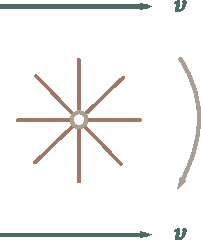
\includegraphics[scale=1]{figures/ch_01/fig_1_30.pdf}
			\caption[]{}
			\label{fig:1_30}
		\end{center}
	\end{minipage}
	\hspace{-0.1cm}
	\begin{minipage}[t]{0.5\linewidth}
		\begin{center}
			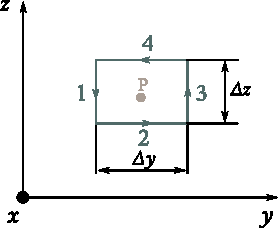
\includegraphics[scale=1]{figures/ch_01/fig_1_31.pdf}
			\caption[]{}
			\label{fig:1_31}
		\end{center}
	\end{minipage}
\vspace{-0.4cm}
\end{figure}

The difference $a_{z,3}-a_{z,1}$ is the increment of the average value of $a_z$ on the section $\Delta{z}$ when this section is displaced in the direction of the $y$-axis by $\Delta{y}$. Owing to the smallness of $\Delta{y}$ and $\Delta{z}$, this increment can be represented in the form $(\diffinpartial{a_z}{y})\Delta{y}$, where the value of $\diffinpartial{a_z}{y}$ is taken for point P\footnote{The inaccuracy which we tolerate here vanishes when the contour shrinks to point P in the limit transition.}. Similarly, the difference $a_{y,4}-a_{y,2}$ can be represented in the form $(\diffinpartial{a_y}{z})\Delta{z}$.
Using these expressions in \eqn{1_91} and putting the common factor outside the parentheses, we get the following expression for the circulation:
\begin{equation*}
	\parenthesis{\diffpartial{a_z}{y} - \diffpartial{a_y}{z}} \Delta{y}\Delta{z} = \parenthesis{\diffpartial{a_z}{y} - \diffpartial{a_y}{z}} \Delta{S}
\end{equation*}

\noindent
where $\Delta{S}$ is the area of the contour. Dividing the circulation by $\Delta{S}$, we find the expression for the projection of $\curl{\vec{a}}$ onto the $x$-axis:
\begin{equation}\label{eq:1_92}
	(\curl{\vec{a}})_x = \diffpartial{a_z}{y} - \diffpartial{a_y}{z}.
\end{equation}

\noindent
We can find by similar reasoning that
\begin{align}
	(\curl{\vec{a}})_y &= \diffpartial{a_x}{z} - \diffpartial{a_z}{x}, \label{eq:1_93}\\
	(\curl{\vec{a}})_z &= \diffpartial{a_y}{x} - \diffpartial{a_x}{y}. \label{eq:1_94}
\end{align}

It is easy to see that any of the equations \eqref{eq:1_92}-\eqref{eq:1_94} can be obtained from the preceding one [\eqn{1_94} should be considered as the preceding one for \eqn{1_94}] by the so-called cyclic transposition of the coordinates, \ie, by replacing the coordinates according to the scheme
\begin{equation*}
	\begin{tikzcd}[column sep=small]
x \arrow[rr, bend left] &           & y \arrow[ld, bend left] \\
                        & z \arrow[lu, bend left] &
\end{tikzcd}
\end{equation*}

Thus, the curl of the vector $\vec{a}$ is determined in the Cartesian coordinate system by the following expression:
\begin{equation}\label{eq:1_95}
	\curl{\vec{a}} = \vecuni{x}\parenthesis{\diffpartial{a_z}{y} - \diffpartial{a_y}{z}} + \vecuni{y}\parenthesis{\diffpartial{a_x}{z} - \diffpartial{a_z}{x}} + \vecuni{z}\parenthesis{\diffpartial{a_y}{x} - \diffpartial{a_x}{y}}.
\end{equation}

\noindent
Below we shall indicate a more elegant way of writing this expression.

\textbf{Stokes' Theorem.} Knowing the curl of the vector $\vec{a}$ at every point of surface $S$ (not necessarily plane), we can calculate the circulation of this vector around contour $\Gamma$ enclosing $S$ (the contour may also not be plane). For this purpose, we divide the surface into very small elements $\Delta{S}$. Owing to their smallness, these elements can be considered as plane. Therefore in accordance with \eqn{1_90}, the circulation of the vector $\vec{a}$ around the contour bounding $\Delta{S}$ can be written in the form
\begin{equation}\label{eq:1_96}
	\Delta{C} \approx (\curl{\vec{a}})_n \Delta{S} = \curl{\vec{a}} \ccdot \Delta{\vec{S}}
\end{equation}

\noindent
where $\hatvec{n}$ is a positive normal to surface element $\Delta{S}$.

In accordance with \eqn{1_88}, summation of expression \eqref{eq:1_96} over all the $\Delta{S}$'s yields the circulation of the vector $\vec{a}$ around contour $\Gamma$ enclosing $S$:
\begin{equation*}
	C = \sum\Delta{C} \approx \sum\curl{\vec{a}} \ccdot \Delta{\vec{S}}.
\end{equation*}

\noindent
Performing a limit transition in which all the $\Delta{S}$'s shrink to zero (their number grows unlimitedly), we arrive at the equation
\begin{equation}\label{eq:1_97}
	\oint_{\Gamma} \vec{a}\ccdot\deriv{\vec{l}} = \int_S (\curl{\vec{a}}) \ccdot \Delta{\vec{S}}.
\end{equation}

\noindent
Equation \eqref{eq:1_97} is called \textbf{Stokes' theorem}. Its meaning is that the circulation of the vector $\vec{a}$ around an arbitrary contour $\Gamma$ equals the flux of the vector $\curl{\vec{a}}$ through the arbitrary surface $S$ surrounded by the given contour.

\textbf{The Del Operator}. Writing of the formulas of vector analysis is simplified quite considerably if we introduce a vector differential operator designated by the symbol $\nabla$ (nabla or del) and called the \textbf{del operator} or the \textbf{Hamiltonian operator}. This operator denotes a vector with the components $\diffinpartial{}{x}$, $\diffinpartial{}{y}$ and $\diffinpartial{}{z}$. Consequently,
\begin{equation}\label{eq:1_98}
	\nabla = \vecuni{x}\diffpartial{}{x} + \vecuni{y}\diffpartial{}{y} + \vecuni{z}\diffpartial{}{z}.
\end{equation}

\noindent
This vector has no meaning by itself. It acquires a meaning in combination with the scalar or vector function by which it is symbolically multiplied. Thus, if we multiply the vector $\nabla$ by the scalar $\varphi$ we obtain the vector
\begin{equation}\label{eq:1_99}
	\gradop{\varphi} = \vecuni{x}\diffpartial{\varphi}{x} + \vecuni{y}\diffpartial{\varphi}{y} + \vecuni{z}\diffpartial{\varphi}{z}
\end{equation}

\noindent
which is the gradient of the function $\varphi$ [see \eqn{1_68}].

The scalar product of the vectors $\nabla$ and $\vec{a}$ gives the scalar
\begin{equation}\label{eq:1_100}
	\divop{\vec{a}} = \nabla_{x}a_{x} + \nabla_{y}a_{y} + \nabla_{z}a_{z}
\end{equation}

\noindent
which we can see to be the divergence of the vector $\vec{a}$ [see \eqn{1_81}].

Finally, the vector product of the vectors $\nabla$ and $\vec{a}$ gives a vector with the components $(\curlop{\vec{a}})_x=\nabla_{y}a_{z} - \nabla_{z}a_{y}=\diffinpartial{a_z}{y}-\diffinpartial{a_y}{z}$, etc., that coincide with the components of $\curl{\vec{a}}$ [see Eqs. \eqref{eq:1_92}-\eqref{eq:1_94}]. Hence, using the writing of a vector product with the aid of a determinant, we have
\begin{equation}\label{1_101}
	\curl{\vec{a}} = \curlop{\vec{a}} = \begin{vmatrix}
	\vecuni{x} & \vecuni{y} & \vecuni{z}\\
	\diffpartial{}{x} & \diffpartial{}{y} & \diffpartial{}{z}\\
	a_x & a_y & a_z
	\end{vmatrix}.
\end{equation}

Thus, there are two ways of denoting the gradient, divergence, and curl:
\begin{equation*}
	\gradop{\varphi}\equiv\grad{\varphi},\quad \divop{\vec{a}}\equiv\diverg{\vec{a}},\quad \curlop{\vec{a}}\equiv\curl{\vec{a}}.
\end{equation*}

\noindent
The use of the del symbol has a number of advantages. We shall therefore use such symbols in the following. One must accustom oneself to identify the symbol $\gradop{\varphi}$ with the words ``gradient of phi'' (\ie, to say not ``del phi'', but ``gradient of phi''), the symbol $\divop{\vec{a}}$ with the words ``divergence of a'' and, finally, the symbol $\curlop{\vec{a}}$ with the words ``curl of a''.

When using the vector $\nabla$, one must remember that it is a differential operator acting on all the functions to the right of it. Consequently, in transforming expressions including $\nabla$, one must take into consideration both the rules of vector algebra and those of differential calculus. For example, the derivative of the product of the functions $\varphi$ and $\psi$ is
\begin{equation*}
	(\varphi\psi)' = \varphi'\psi + \varphi\psi'.
\end{equation*}

\noindent
Accordingly,
\begin{equation}\label{eq:1_102}
	\grad{(\varphi\psi)} = \gradop{(\varphi\psi)} = \psi\gradop{\varphi} + \varphi\gradop{\psi} = \psi\,\grad{\varphi} + \varphi\,\grad{\psi}.
\end{equation}

\noindent
Similarly,
\begin{equation}\label{eq:1_103}
	\diverg{(\varphi\vec{a})} = \divop{(\varphi\vec{a})} = \vec{a}\ccdot(\gradop{\varphi}) + \varphi(\divop{\vec{a}}).
\end{equation}

The gradient of a function $\varphi$ is a vector function. Therefore, the divergence and curl operations can be performed with it:
\begin{align}
	\diverg{\grad{\varphi}} &= \divop{\gradop{\varphi}} = (\divop{\nabla})\varphi = \parenthesis{\nabla_x^2 + \nabla_y^2 + \nabla_z^2}\varphi\nonumber\\
	&= \diffsecpartial{\varphi}{x} + \diffsecpartial{\varphi}{y} + \diffsecpartial{\varphi}{z} = \upDelta{\varphi}\label{eq:1_104}
\end{align}

\noindent
($\upDelta$ is the Laplacian operator)
\begin{equation}\label{eq:1_105}
	\curl{\grad{\varphi}} = \curlop{(\gradop{\varphi})} = (\curlop{\nabla})\varphi
\end{equation}

\noindent
(we remind our reader that the vector product of a vector and itself is zero).

Let us apply the divergence and curl operations to the function $\curl{\vec{a}}$:
\begin{equation}\label{eq:1_106}
	\diverg{\curl{\vec{a}}} = \divop{\curlop{\vec{a}}} = 0
\end{equation}

\noindent
(a scalar triple product equals the volume of a parallelepiped constructed on the vectors being multiplied (see Vol. I, p. 22); if two of these vectors coincide, the volume of the parallelepiped equals zero):
\begin{equation}\label{eq:1_107}
	\curl{\curl{\vec{a}}} = \curlop{(\curlop{\vec{a}})} = \gradop{(\divop{\vec{a}})} - (\divop{\nabla})\vec{a} = \grad{\diverg{\vec{a}}} - \upDelta{\vec{a}}
\end{equation}

\noindent
[we have used Eq. (1.35) of Vol. I, namely, $\vec{a}\times\vec{b}\times\vec{c} = \vec{b}(\vecdot{a}{c}) - \vec{c}(\vecdot{a}{b})$].

Equation \eqref{eq:1_106} signifies that the field of a curl has no sources. Hence, the lines of the vector $\curl{\vec{a}}$ have neither a beginning nor an end. It is exactly for this reason that the flux of a curl through any surface $S$ resting on the given contour $\Gamma$ is the same [see \eqn{1_97}).

We shall note in concluding that when the del operator is used, Eqs. \eqref{eq:1_82} and \eqref{eq:1_97} can be given the form
\begin{align}
	\oint_S \vec{a} \ccdot \deriv{\vec{S}} &= \oint_V \divop{\vec{a}}\, \deriv{V},\quad\quad\! \text{(the Ostrogradsky-Gauss theorem)}\label{eq:1_108}\\
	\oint_{\Gamma} \vec{a} \ccdot \deriv{\vec{l}} &= \int_S (\curlop{\vec{a}}) \ccdot \deriv{\vec{S}}.\quad \text{(Stokes' theorem)}\label{eq:1_109}
\end{align}

\section{Circulation and Curl of an Electrostatic Field}\label{sec:1_12}

We established in \sect{1_6} that the forces acting on the charge $q$ in an electrostatic field are conservative. Hence, the work of these forces on any closed path $\Gamma$ is zero:
\begin{equation*}
	A = \oint_{\Gamma} q\vec{E} \ccdot \deriv{\vec{l}} = 0.
\end{equation*}

\noindent
Cancelling $q$, we get
\begin{equation}\label{eq:1_110}
	\oint_{\Gamma} \vec{E} \ccdot \deriv{\vec{l}} = 0
\end{equation}

\noindent
(compare with \eqn{1_46}].

The integral in the left-hand side of \eqn{1_110} is the circulation of the vector $\vec{E}$ around contour $\Gamma$ [see expression \eqref{eq:1_80}]. Thus, \textit{an electrostatic field is characterized by the fact that the circulation of the strength (intensity) vector of this field around any closed contour equals zero}.

Let us take an arbitrary surface $S$ resting on contour $\Gamma$ for which the circulation is calculated (\fig{1_32}). According to Stokes's
theorem [see \eqn{1_109}], the integral of $\curl{\vec{E}}$ taken over this surface equals the circulation of the vector $\vec{E}$ around contour $\Gamma$:
\begin{equation}\label{eq:1_111}
	\int_S (\curlop{\vec{E}}) \ccdot \deriv{\vec{S}} = \oint_{\Gamma} \vec{E} \ccdot \deriv{\vec{l}}.
\end{equation}

\noindent
Since the circulation equals zero, we arrive at the conclusion that
\begin{equation*}
	\int_S (\curlop{\vec{E}}) \ccdot \deriv{\vec{S}} = 0.
\end{equation*}

\noindent
This condition must be observed for any surface $S$ resting on arbitrary contour $\Gamma$. This is possible only if the curl of the vector $\vec{E}$ at every point of the field equals zero:
\begin{equation}\label{eq:1_112}
	\curlop{\vec{E}} = 0.
\end{equation}

\begin{figure}[t]
	\begin{minipage}[t]{0.5\linewidth}
		\begin{center}
			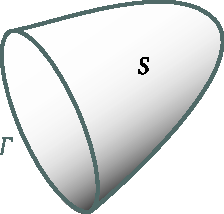
\includegraphics[scale=1]{figures/ch_01/fig_1_32.pdf}
			\caption[]{}
			\label{fig:1_32}
		\end{center}
	\end{minipage}
	\hspace{-0.1cm}
	\begin{minipage}[t]{0.5\linewidth}
		\begin{center}
			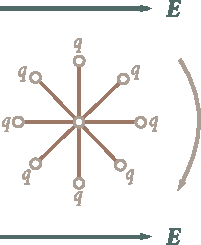
\includegraphics[scale=1]{figures/ch_01/fig_1_33.pdf}
			\caption[]{}
			\label{fig:1_33}
		\end{center}
	\end{minipage}
\vspace{-0.4cm}
\end{figure}

By analogy with the fan impeller shown in \fig{1_25}, let us imagine an electrical ``impeller'' in the form of a light hub with spokes whose ends carry identical positive charges $q$ (\fig{1_33}; the entire arrangement must be small in size). At the points of an electric field where $\curl{\vec{E}}$ differs from zero, such an impeller would rotate with an acceleration that is the greater, the larger is the projection of the curl onto the impeller axis. For an electrostatic field, such an imaginary arrangement would not rotate with any orientation of its axis.

Thus, a feature of an electrostatic field is that it is a non-circuital one. We established in the preceding section that the curl of the gradient of a scalar function equals zero [see expression \eqref{eq:1_96}]. Therefore, the equality to zero of $\curl{\vec{E}}$ at every point of a field makes it possible to represent $\vec{E}$ in the form of the gradient of a scalar function $\varphi$ called the potential. We have already considered this representation in \sect{1_8} [see \eqn{1_41}; the minus sign in this equation was taken from physical considerations].

We can immediately conclude from the need to observe condition \eqref{eq:1_110} that the existence of an electrostatic field of the kind shown in \fig{1_34} is impossible. Indeed, for such a field, the circulation around the contour shown by the dash line would differ from zero, which contradicts condition \eqref{eq:1_110}. It is also impossible for a field differing from zero in a restricted volume to be homogeneous throughout this volume (\fig{1_35}). In this case, the circulation around the contour shown by the dash line would differ from zero.

\begin{figure}[t]
	\begin{minipage}[t]{0.36\linewidth}
		\begin{center}
			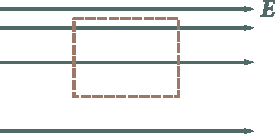
\includegraphics[scale=0.93]{figures/ch_01/fig_1_34.pdf}
			\caption[]{}
			\label{fig:1_34}
		\end{center}
	\end{minipage}
	% \hspace{-0.05cm}
	\hfill{ }
	\begin{minipage}[t]{0.2\linewidth}
		\begin{center}
			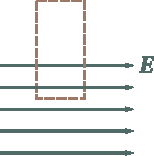
\includegraphics[scale=0.93]{figures/ch_01/fig_1_35.pdf}
			\caption[]{}
			\label{fig:1_35}
		\end{center}
	\end{minipage}
	% \hspace{-0.05cm}
	\hfill{ }
	\begin{minipage}[t]{0.37\linewidth}
		\begin{center}
			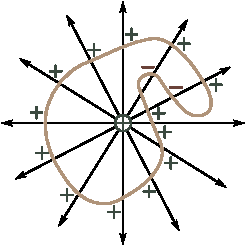
\includegraphics[scale=0.95]{figures/ch_01/fig_1_36.pdf}
			\caption[]{}
			\label{fig:1_36}
		\end{center}
	\end{minipage}
\vspace{-0.5cm}
\end{figure}

\section{Gauss's Theorem}\label{sec:1_13}

We established in the preceding section what the curl of an electrostatic field equals. Now let us find the divergence of a field. For this purpose, we shall consider the field of a point charge $q$ and calculate the flux of the vector $\vec{E}$ through closed surface $S$ surrounding the charge (\fig{1_36}). We showed in \sect{1_5} that the number of lines of the vector $\vec{E}$ beginning at a point charge $+q$ or terminating at a charge $-q$ numerically equals $q/\varepsilon_0$.

By \eqn{1_77}, the flux of the vector $\vec{E}$ through any closed surface equals the number of lines coming out, \ie, beginning on the
charge, if it is positive, and the number of lines entering the surface, \ie, terminating on the charge, if it is negative. Taking into account that the number of lines beginning or terminating at a point charge numerically equals $q/\varepsilon_0$ (see \sect{1_5}), we can write that
\begin{equation}\label{eq:1_113}
	\Phi_E = \frac{q}{\varepsilon_0}.
\end{equation}

\noindent
The sign of the flux coincides with that of the charge $q$. The dimensions of both sides of \eqn{1_113} are identical.

Now let us assume that a closed surface surrounds $N$ point charges $q_1, q_2, \ldots, q_N$. On the basis of the superposition principle, the strength $\vec{E}$ of the field set up by all the charges equals the sum of the strengths $\vec{E}_i$  set up by each charge separately: $\vec{E}=\sum_i\vec{E}_i$. Hence,
\begin{equation*}
	\Phi_E = \oint_S \vec{E}\ccdot\deriv{\vec{S}} = \oint_S \parenthesis{\sum_i\vec{E}_i}\ccdot\deriv{\vec{S}} = \sum_i\oint_S\vec{E}_i\ccdot\deriv{\vec{S}}.
\end{equation*}

\noindent
Each of the integrals inside the sum sign equals $q_i/\varepsilon_0$. Therefore,
\begin{equation}\label{eq:1_114}
	\Phi_E = \oint_S \vec{E}\ccdot\deriv{\vec{S}} = \frac{1}{\varepsilon_0} \sum_{i=1}^N q_i.
\end{equation}

\noindent
The statement we have proved is called \textbf{Gauss's theorem}. According to it, \textit{the flux of an electric field strength vector through a closed surface equals the algebraic sum of the charges enclosed by this surface divided by $\varepsilon_0$}.

When considering fields set up by macroscopic charges (\ie, charges formed by an enormous number of elementary charges), the discrete structure of these charges is disregarded, and they are considered to be distributed in space continuously with a finite density everywhere. The \textbf{volume density of a charge} $\rho$ is determined by analogy with the density of a mass as the ratio of the charge $\deriv{q}$ to the infinitely small (physically) volume $\deriv{V}$ containing this charge:
\begin{equation}\label{eq:1_115}
	\rho = \diff{q}{V}.
\end{equation}

\noindent
In the given case by an infinitely small (physically) volume, we must understand a volume which on the one hand is sufficiently small for the density within its limits to be considered identical, and on the other is sufficiently great for the discreteness of the charge not to manifest itself.

Knowing the charge density at every point of space, we can find the total charge surrounded by closed surface $S$. For this purpose, we must calculate the integral of $\rho$ with respect to the volume enclosed by the surface:
\begin{equation*}
	\sum_i q_i = \int_V \rho\,\deriv{V}.
\end{equation*}

\noindent
Thus, \eqn{1_114} can be written in the form
\begin{equation}\label{eq:1_116}
	\oint_S \vec{E}\ccdot\deriv{\vec{S}} = \frac{1}{\varepsilon_0} \int_V \rho\,\deriv{V}.
\end{equation}

Replacing the surface integral with a volume one in accordance with \eqn{1_108}, we have
\begin{equation*}
	\int_V \divop{\vec{E}}\,\deriv{V} = \frac{1}{\varepsilon_0} \int_V \rho\,\deriv{V}.
\end{equation*}

\noindent
The relation which we have arrived at must be observed for any arbitrarily chosen volume $V$. This is possible only if the values of the integrands for every point of space are the same. Hence, the divergence of the vector $\vec{E}$ is associated with the density of the charge at the same point by the equation
\begin{equation}\label{eq:1_117}
	\divop{\vec{E}} = \frac{1}{\varepsilon_0} \rho.
\end{equation}

\noindent
This equation expresses Gauss's theorem in the differential form.

For a flowing liquid, $\divop{\vec{v}}$ gives the unit power of the sources of the liquid at a given point. By analogy, charges are said to be sources of an electric field.

\section{Calculating Fields with the Aid of Gauss's Theorem}\label{sec:1_14}

Gauss's theorem permits us in a number of cases to find the strength of a field in a much simpler way than by using \eqn{1_15} for the field strength of a point charge and the field superposition principle. We shall demonstrate the possibilities of Gauss's theorem by employing a few examples that will be useful for our further exposition. Before starting on our way, we shall introduce the concepts of surface and linear charge densities.

If a charge is concentrated in a thin surface layer of the body carrying the charge, the distribution of the charge in space can be characterized by the surface density $\sigma$, which is determined by the expression
\begin{equation}\label{eq:1_118}
	\sigma = \diff{q}{S}.
\end{equation}

\noindent
Here $\deriv{q}$ is the charge contained in the layer of area $\deriv{S}$. By $\deriv{S}$ is meant an infinitely small (physically) section of the surface.

If a charge is distributed over the volume or surface of a cylindrical body (uniformly in each section), the linear charge density is used, \ie,
\begin{equation}\label{eq:1_119}
	\lambda = \diff{q}{l}
\end{equation}

\noindent
where $\deriv{l}$ is the length of an infinitely small (physically) segment of the cylinder, and $\deriv{q}$ is the charge concentrated on this segment.

\textbf{Field of an Infinite Homogeneously Charged Plane.} Assume that the surface charge density at all points of a plane is identical and equal to $\sigma$; for definiteness we shall consider the charge to be positive. It follows from considerations of symmetry that the field strength at any point is directed at right angles to the plane. Indeed, since the plane is infinite and charged homogeneously, there is no reason why the vector $\vec{E}$ should deflect to a side from a normal to the plane. It is further evident that at points symmetrical relative to the plane, the field strength is identical in magnitude and opposite in direction.

\begin{figure}[t]
	\begin{minipage}[t]{0.5\linewidth}
		\begin{center}
			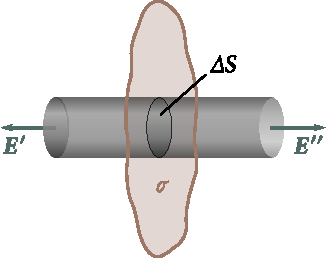
\includegraphics[scale=1]{figures/ch_01/fig_1_37.pdf}
			\caption[]{}
			\label{fig:1_37}
		\end{center}
	\end{minipage}
	\hspace{-0.05cm}
	\begin{minipage}[t]{0.5\linewidth}
		\begin{center}
			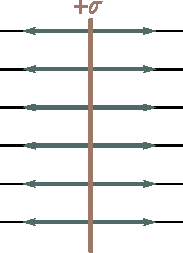
\includegraphics[scale=1]{figures/ch_01/fig_1_38.pdf}
			\caption[]{}
			\label{fig:1_38}
		\end{center}
	\end{minipage}
\vspace{-0.4cm}
\end{figure}

Let us imagine mentally a cylindrical surface with generatrices perpendicular to the plane and bases of a size $\Delta{S}$ arranged symmetrically relative to the plane (\fig{1_37}). Owing to symmetry, we have $E'=E''=E$. We shall apply Gauss's theorem to the surface. The flux through the side part of the surface will be absent because $E_n$ at each point of it is zero. For the bases, $E_n$ coincides with $E$. Hence, the total flux through the surface is $2E\Delta{S}$. The surface encloses the charge $\sigma\Delta{S}$. According to Gauss's theorem, the condition must be observed that
\begin{equation*}
	2E\Delta{S} = \frac{\sigma\Delta{S}}{\varepsilon_0}
\end{equation*}

\noindent
whence
\begin{equation}\label{eq:1_120}
	E = \frac{\sigma}{2\varepsilon_0}.
\end{equation}

\noindent
The result we have obtained does not depend on the length of the cylinder. This signifies that at any distances from the plane, the field strength is identical in magnitude. The field lines are shown in \fig{1_38}. For a negatively charged plane, the result will be the same except for the reversal of the direction of the vector $\vec{E}$ and the field lines.

If we take a plane of finite dimensions, for instance a charged thin plate\footnote{For a plate, by $\sigma$ in \eqn{1_120} should be understood the charge concentrated on \SI{1}{\metre\squared} of the plate over its entire thickness. In metal bodies, the charge is distributed over the external surface. Therefore by $\sigma$ we should understand the double value of the charge density on the surfaces surrounding the metal plate.}, then the result obtained above will hold only for points, the distance to which from the edge of the plate considerably exceeds the distance from the plate itself (in \fig{1_39} the region containing such points is outlined by a dash line). At points at an increasing distance from the plane or approaching its edges, the field will differ more and more from that of an infinitely charged plane. It is easy to imagine the nature of the field at great distances if we take into account that at distances considerably exceeding the dimensions of the plate, the field it sets up can be treated as that of a point charge.

\textbf{Field of Two Uniformly Charged Planes.} The field of two parallel infinite planes carrying opposite charges with a constant surface density $\sigma$ identical in magnitude can be found by superposition of the fields produced by each plane separately (\fig{1_40}). In the region between the planes, the fields being added have the same direction, so that the resultant field strength is
\begin{equation}\label{eq:1_121}
	E = \frac{\sigma}{\varepsilon_0}.
\end{equation}

\noindent
Outside the volume bounded by the planes, the fields being added have opposite directions so that the resultant field strength equals zero.

\begin{figure}[t]
	\begin{minipage}[t]{0.5\linewidth}
		\begin{center}
			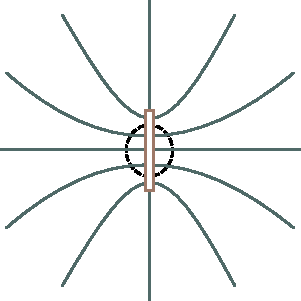
\includegraphics[scale=1]{figures/ch_01/fig_1_39.pdf}
			\caption[]{}
			\label{fig:1_39}
		\end{center}
	\end{minipage}
	\hspace{-0.05cm}
	\begin{minipage}[t]{0.5\linewidth}
		\begin{center}
			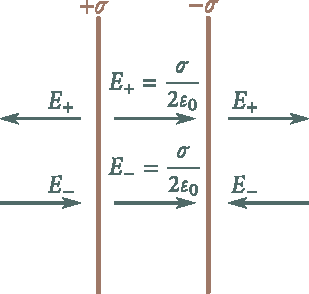
\includegraphics[scale=1]{figures/ch_01/fig_1_40.pdf}
			\caption[]{}
			\label{fig:1_40}
		\end{center}
	\end{minipage}
\vspace{-0.55cm}
\end{figure}

Thus, the field is concentrated between the planes. The field strength at all points of this region is identical in value and in direction; consequently, the field is homogeneous. The field lines are a collection of parallel equispaced straight lines.

The result we have obtained also holds approximately for planes of finite dimensions if the distance between them is much smaller than their linear dimensions (a parallel-plate capacitor). In this case, appreciable deviations of the field from homogeneity are observed only near the edges of the plates (\fig{1_41}).

\textbf{Field of an Infinite Charged Cylinder.} Assume that the field is produced by an infinite cylindrical surface of radius $R$ whose charge has a constant surface density $\sigma$. Considerations of symmetry show that the field strength at any point must be directed along a radial line perpendicular to the cylinder axis, and that the magnitude of the strength can depend only on the distance $r$ from the cylinder axis. Let us mentally imagine a coaxial closed cylindrical surface of radius $r$ and height $h$ with a charged surface (\fig{1_42}). For the bases of the cylinder, we have $E_n=0$, for the side surface $E_n=E(r)$ (the charge is assumed to be positive). Hence, the flux of the vector $\vec{E}$ through the surface being considered is $E(r)\times 2\pi rh$. If $r>R$, the charge $q=\lambda h$ (where $\lambda$ is the linear charge density) will get into the surface. Applying Gauss's theorem, we find that
\begin{equation*}
	E(r)\times 2\pi rh = \frac{2\lambda}{\varepsilon_0}.
\end{equation*}

\noindent
Hence,
\begin{equation}\label{eq:1_122}
	E(r) = \frac{1}{2\pi\varepsilon_0}\frac{\lambda}{r}\quad (r\geqslant R).
\end{equation}

\noindent
If $r<R$, the closed surface being considered contains no charges inside, owing to which $E(r)=0$.

\begin{figure}[t]
	\begin{minipage}[t]{0.35\linewidth}
		\begin{center}
			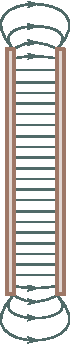
\includegraphics[scale=1]{figures/ch_01/fig_1_41.pdf}
			\caption[]{}
			\label{fig:1_41}
		\end{center}
	\end{minipage}
	\hspace{-0.05cm}
	\begin{minipage}[t]{0.65\linewidth}
		\begin{center}
			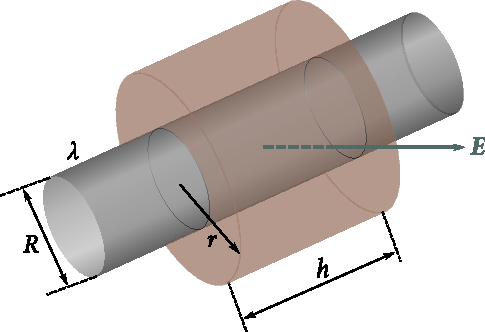
\includegraphics[scale=0.95]{figures/ch_01/fig_1_42.pdf}
			\caption[]{}
			\label{fig:1_42}
		\end{center}
	\end{minipage}
\vspace{-0.4cm}
\end{figure}

Thus, there is no field inside a uniformly charged cylindrical surface of infinite length. The field strength outside the surface is determined by the linear charge density $\lambda$ and the distance $r$ from the cylinder axis.

The field of a negatively charged cylinder differs from that of a positively charged one only in the direction of the vector $\vec{E}$. A glance at \eqn{1_122} shows that by reducing the cylinder radius $R$ (with a constant linear charge density $\lambda$), we can obtain a field with a very great strength near the surface of the cylinder.

Introducing $\lambda=2\pi R\sigma$ into \eqn{1_122} and assuming that $r=R$, we get the following value for the field strength in direct proximity to the surface of a cylinder:
\vspace{-12pt}
\begin{equation}\label{eq:1_123}
	E(R) = \frac{\sigma}{\varepsilon_0}.
\end{equation}

The superposition principle makes it simple to find the field of two coaxial cylindrical surfaces carrying a linear charge density $\lambda$ of the same magnitude, but of opposite signs (\fig{1_43}). There is no field inside the smaller and outside the larger cylinders. The field strength in the gap between the cylinders is determined by \eqn{1_122}. This also holds for cylindrical surfaces of a finite length if the gap between the surfaces is much smaller than their length (a cylindrical capacitor). Appreciable deviations from the field of surfaces of an infinite length will be observed only near the edges of the cylinders.

\begin{figure}[t]
	\begin{center}
		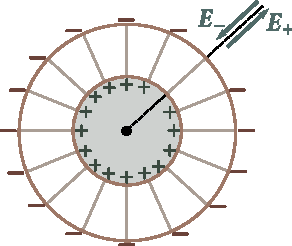
\includegraphics[scale=1]{figures/ch_01/fig_1_43.pdf}
		\caption[]{}
		\label{fig:1_43}
	\end{center}
	\vspace{-0.8cm}
\end{figure}

\textbf{Field of a Charged Spherical Surface.} The field produced by a spherical surface of radius $R$ whose charge has a constant surface density $\sigma$ will obviously be a centrally symmetrical one. This signifies that the direction of the vector $\vec{E}$ at any point passes through the centre of the sphere, while the magnitude of the field strength is a function of the distance $r$ from the centre of the sphere. Let us imagine a surface of radius $r$ that is concentric with the charged sphere. For all points of this surface, $E_n=E(r)$. If $r>R$, the entire charge $q$ distributed over the sphere will be inside the surface. Hence,
\begin{equation*}
	E(r)\times 4\pi r^2 = \frac{q}{\varepsilon_0}
\end{equation*}

\noindent
whence
\begin{equation}\label{eq:1_124}
	E(r) = \frac{1}{4\pi\varepsilon_0}\frac{q}{r^2}.\quad (r\geqslant R)
\end{equation}

A spherical surface of radius $r$ less than $R$ will contain no charges, owing to which for $r<R$ we get $E(r)=0$.

Thus, there is no field inside a spherical surface whose charge has a constant surface density $\sigma$. Outside this surface, the field is identical with that of a point charge of the same magnitude at the
centre of the sphere.

Using the superposition principle, it is easy to show that the field of two concentric spherical surfaces (a spherical capacitor) carrying charges $+q$ and $-q$ that are identical in magnitude and opposite in sign is concentrated in the gap between the surfaces, the magnitude of the field strength in the gap being determined by \eqn{1_124}.

\textbf{Field of a Volume-Charged Sphere.} Assume that a sphere of radius $R$ has a charge with a constant volume density $\rho$. The field in this case has central symmetry. It is easy to see that the same result is obtained for the field outside the sphere [see \eqn{1_124}] as for a sphere with a surface charge. The result will be different for points inside the sphere, however. A spherical surface of radius $r$ ($r<R$) contains a charge equal to $\rho\times 4\pi r^3/3$. Therefore, Gauss's theorem for such a surface will be written as follows:
\begin{equation*}
	E(r)\times 4\pi r^2 = \frac{1}{\varepsilon_0}\rho \frac{4}{3}\pi r^3.
\end{equation*}

\noindent
Hence, substituting $q/(4\pi R^3/3)$ for $\rho$, we get
\begin{equation}\label{eq:1_125}
	E(r) = \frac{1}{4\pi\varepsilon_0}\frac{q}{R^3}r.\quad (r\leqslant R)
\end{equation}

Thus, the field strength inside a sphere grows linearly with the distance $r$ from the centre of the sphere. Outside the sphere, the field strength diminishes according to the same law as for the field of a point charge.
